% libroResMat2
% Copyright (C) 2020  J.M. Perez Zerpa, et. al.
%
% This program is free software: you can redistribute it and/or modify
% it under the terms of the GNU General Public License as published by
% the Free Software Foundation version 3 of the License.
%
% This program is distributed in the hope that it will be useful,
% but WITHOUT ANY WARRANTY; without even the implied warranty of
% MERCHANTABILITY or FITNESS FOR A PARTICULAR PURPOSE. See the
% GNU General Public License for more details.
%
% You should have received a copy of the GNU General Public License
% along with this program.  If not, see <http://www.gnu.org/licenses/>.

\chapter{Estabilidad Estructural}

En esta unidad temática se consideran nuevas referencias, dado que se debe introducir un concepto fundamentalmente diferente al resto de las unidades temáticas. %
%
La hipótesis fundamental modificada: es que el equilibrio deja de realizarse en la configuración de referencia para realizarlo en una configuración deformada (bajo hipótesis de pequeños giros), permitiendo modelar el fenómeno de \textit{inestabilidad estructural}. %
%
Las principales referencias utilizadas son \citep{yoo2011,Bazzano2017}.

\section{Introduccion} 

El inicio del estudio de la estabilidad elástica de elementos estructurales se remonta al trabajo de Leonard Euler, quien en 1757 presentó un resultado que sigue siendo hoy en día central para el análisis y diseño de columnas esbeltas. %
%
Euler determinó que, para una columna con proporcionalidad entre momento flector y curvatura, existe un valor de compresión crítica a partir de la cual, la columna pierde la estabilidad. %
%
El lector interesado podrá ver más detalles del trabajo pionero de Euler en \citep{Timoshenko1953}.

El fenómeno de la inestabilidad elástica se tornó un tema cada vez más relevante con la adopción del hierro (y posteriormente el acero) como material de construcción. %
%
Se debe recordar que el primer puente de hierro se construyó en Coalbrookdale, Inglaterra en 1781 y el primer puente de celosía de acero se construyó sobre el río Mississipi, EEUU en 1868.  Estos materiales permitieron la construcción de estructuras con componentes cada vez más esbeltos. 

En este contexto, hubo un número de colapsos debido a fallos por inestabilidad elástica. La clara representación del fenómeno de inestabilidad, así como por sus consecuencias trágicas, hacen de estos fallos casos de estudio típicos para estudiantes de ingeniería. Uno de ellos se dio en 1907 en la construcción del puente sobre el río Quebec, Canadá, mostrado en la Figura~\ref{fig:Quebec}. La estructura del puente contaba con ménsulas balanceadas y un vano libre de 549 m. Una serie de errores, omisiones y malas prácticas llevaron al colapso del puente. En última instancia, el colapso se debió a una falla por inestabilidad de un barra sometida a gran compresión, resultando en la muerte de 75 operarios. Se recomienda leer el artículo publicado por \cite{Brady} para conocer más detalles de este caso.

%\begin{figure}[htb]
%  \centering
%%  AGREGAR FOTO
%  \includegraphics[width=0.95\textwidth]{../../quebec}
%	\caption{Puente Sobre Río Quebec, Canada \citep{Brady}.}
%	\label{fig:Quebec}
%\end{figure}

En tiempos más recientes, una serie de colapsos se dieron en un corto plazo de tiempo en una tipología estructural de puente que se estaba popularizando en ese momento. Los puentes con sección cajón de acero de Milford Haven (1970, Gales) (el cual es mostrado en la Figura~\ref{fig:Milford}), Koblenz (1971, Alemania) y West Gate (1970, Australia) son algunos de los casos en dicha serie de colapsos. En todos ellos, la inestabilidad de las placas de acero que componen los cajones fue un factor determinante en los colapsos. Se hace referencia al articulo de \cite{Firth}\footnote{Disponible en \href{https://www.istructe.org/webtest/files/48/488ca532-a956-4929-9f50-aee0d5317afc.pdf}{www.istructe.org/webtest/files/48/488ca532-a956-4929-9f50-aee0d5317afc.pdf}, ult. acceso 21/Oct/2019} para conocer la historia de dicha tipología, así como la serie de colapsos en la década de los 70.

%\begin{figure}[htb]
%  \centering
%%  AGREGAR FOTO
%  \includegraphics[width=0.8\textwidth]{../../Milford_Haven.png}
%	\caption{Colapso en Milford Haven, Gales \citep{Firth}.}
%	\label{fig:Milford}
%\end{figure}
%
Estos colapsos fueron el disparador de un gran esfuerzo de investigación en estructuras con el objetivo de generar reglas de diseño para evitar nuevos colapsos en esta clase de estructuras. En Inglaterra, dicho impulso resultó en la serie de reglas de diseño conocidas como IDWR, que luego pasaría a formar parte de BS 5400-3, la antigua norma británica para diseño de puentes de acero, hoy reemplazada por el Eurocódigo EN 1993. Dicha investigación avanzó enormemente el entendimiento de cómo se comportan los cajones de acero, en particular la estabilidad de las chapas rigidizadas que los componen. El lector interesado puede leer el reporte de la comisión investigadora del colapso de West Gate\footnote{Disponible en \href{http://www.parliament.vic.gov.au/papers/govpub/VPARL1971-72No2.pdf}{www.parliament.vic.gov.au/papers/govpub/VPARL1971-72No2.pdf}, ult. acceso 21/Oct/2019}, en el cual se puede apreciar la magnitud y complejidad de la estructura que colapsó. 

%\begin{figure}[htb]
%  \centering
%  %\width{0.6\textwidth}
%%  AGREGAR FOTO
%  \includegraphics[width=0.8\textwidth]{../../Westgate.png}
%	\caption{Puente Westgate, Australia. Izquierda: dibujo esquemático de sección cajón. Derecha: cajón durante montaje, observar pandeo de chapa superior.Referencia Informe Royal Commission.}
%	\label{fig:Westgate}
%\end{figure}

Las normas modernas exigen, o permiten, que los problemas comunes de inestabilidad sean considerados mediante reglas relativamente sencillas. Todos los materiales incluyen reglas en sus respectivas normas para la evaluación de la estabilidad estructural, tanto a nivel de componentes así como a nivel global de la estructura. Sin embargo, el diseño de estructuras de acero es el que hace mayor hincapié en este tema, dado que en general dichas estructuras se forman a partir de un gran número de componentes esbeltos. 

A modo de ejemplo, se refiere a la sección E3 de la norma AISC 360-16 o sección 6.3.1 de la norma EN 1993-1-1 para ver el tratamiento de resistencia axial de columnas esbeltas de acero que fallan por inestabilidad. El lector encontrará que las normas hacen referencia a $F_e$ (AISC 360-16) y $N_{cr}$ (EN 1993-1-1) que son escencialmente la carga crítica que Euler descubrió en 1757.

Finalmente, las normas también exigen la evaluación de la estabilidad global de la estructura. El capítulo C de la norma AISC 360-16 trata sobre este tema, mientras que la norma EN 1992-1-1 lo hace en el Anexo H. En pocas palabras, se requiere que el ingeniero evalúe la estabilidad de la estructura en su conjunto y que determine los efectos que puedan surgir de la esbeltez global de la estructura. Estas evaluaciones son parte básica del trabajo del ingeniero que diseña una estructura.


\section{Principio de Mínima Energía Potencial Total}

\subsection{Criterios de equilibrio y estabilidad} 
En la sección 1.2.2 se introdujo el concepto que una estructura satisface las ecuaciones de elasticidad lineal (equilibrio, compatibilidad de deformaciones y relación tensión deformación lineal) si es solución del problema de minimización:

\begin{equation*}
\bfu = \arg\min_{\bfu\in\mcU} \Pi(\bfu)
\end{equation*}

La condición de mínima energía potencial total no solo garantiza equilibrio de las estructuras, sino que también implica la estabilidad de las mismas.

Debe entenderse por estabilidad la propiedad de la estructura de, bajo un cierto conjunto de cargas externas, poder mantenerse arbitrariamente cerca de la configuración de equilibrio al ser sometida a una pequeña perturbación arbitraria.

Para el modelo estructural lineal (i.e. equilibrio en la configuración de referencia, pequeños desplazamientos y material elástico lineal) de estructuras de barras visto en capítulos anteriores, la condición de mínimo requiere que la matriz de rigidez de la estructura $\bfK$ sea definida positiva.

$$\forall \bfu\neq 0 \in \mcU, \bfu \cdot \bfK \bfu > 0$$

Esto se desprende del hecho que la energía potencial total de la estructura es igual a:

$$\Pi(\bfu)= \frac{1}{2} \bfu \cdot \bfK \bfu - \bfF_G \cdot \bfu$$

La condición de mínimo requiere que todos los valores propios de matriz Hessiana de la función $\Pi(\bfu)$ sean positivos. Donde dicha matriz Hessiana igual a $\bfK$ y la condición de valores propios positivos es equivalente a la condición de definida positiva. 

Se puede verificar que para estructuras con condiciones de apoyo suficientes y que no tengan mecanismos internos, se verifica la condición presentada. Con lo cual, se puede concluir que con dichos modelos estructurales lineales, no es posible modelar la inestabilidad elástica de una estructura. Para ello, debemos modificar el modelo estructural y abandonar la hipótesis de equilibrio en la configuración de referencia.
 
%(pmept). Mostrar q lo visto hasta este momento (pequeñas defs y material lineal) resulta en estructuras estables de barras (i.e. una vez impuestos CdB suficientes, K es definida positiva).

\subsection{Tipos de Sistemas Estructurales} 

El estudio de estabilidad elástica mediante el prinicipio de mínima energía potencial total puede realizarse tanto en estructuras discretas como continuas. La diferencia entre un tipo de estructuras y el otro es el espacio $\mcU$ donde buscamos el mínimo de la energía potencial total.

En el caso de estructuras continuas, la configuración deformada de la estructura $\bfu$ se expresa mediante una o más funciones. Se puede decir que la estructura tiene efectivamente infinitos grados de libertad o que $\mcU$ es un espacio de dimensión infinita.

En la \autoref{fig:PandeoContinuo} se pueden ver algunos ejemplos de sistemas estructurales continuos, donde la Figura\autoref{fig:PandeoChapa} representa una chapa sometida a cargas de compresión meridional y la Figura\autoref{fig:PandeoViga} una viga sometida a cargas verticales.

\begin{figure}[htb]
	\centering
\subfloat[Pandeo de Chapa a compresión]{
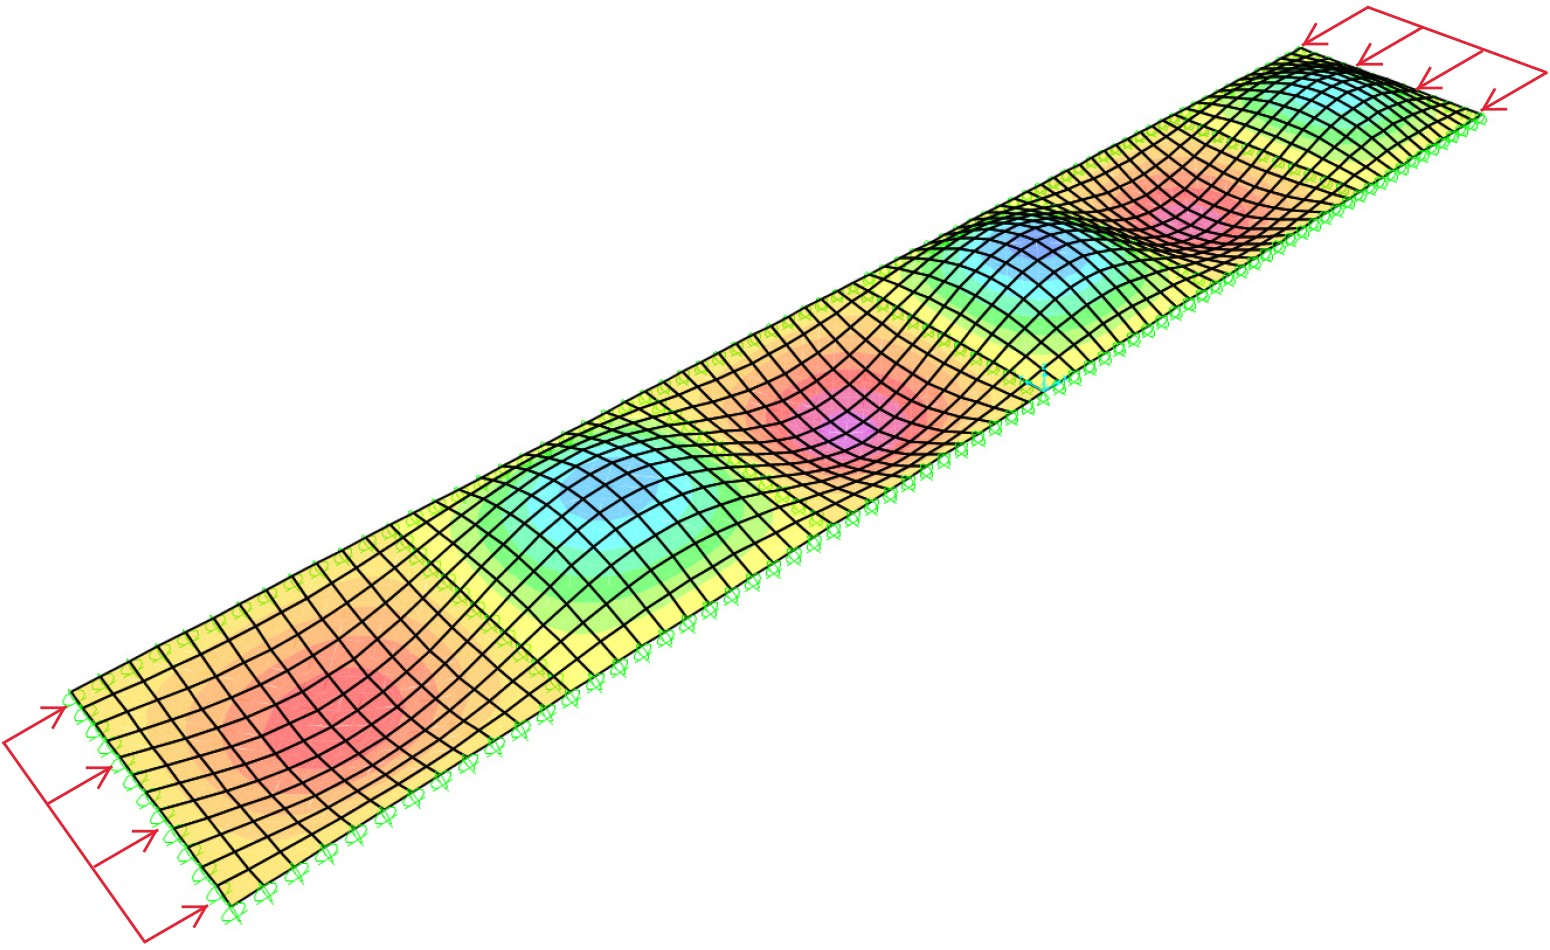
\includegraphics[width=0.45\textwidth]{PandeoChapa}
	\label{fig:PandeoChapa}}
\hspace{1em}
\subfloat[Pandeo lateral de viga por flexión]{
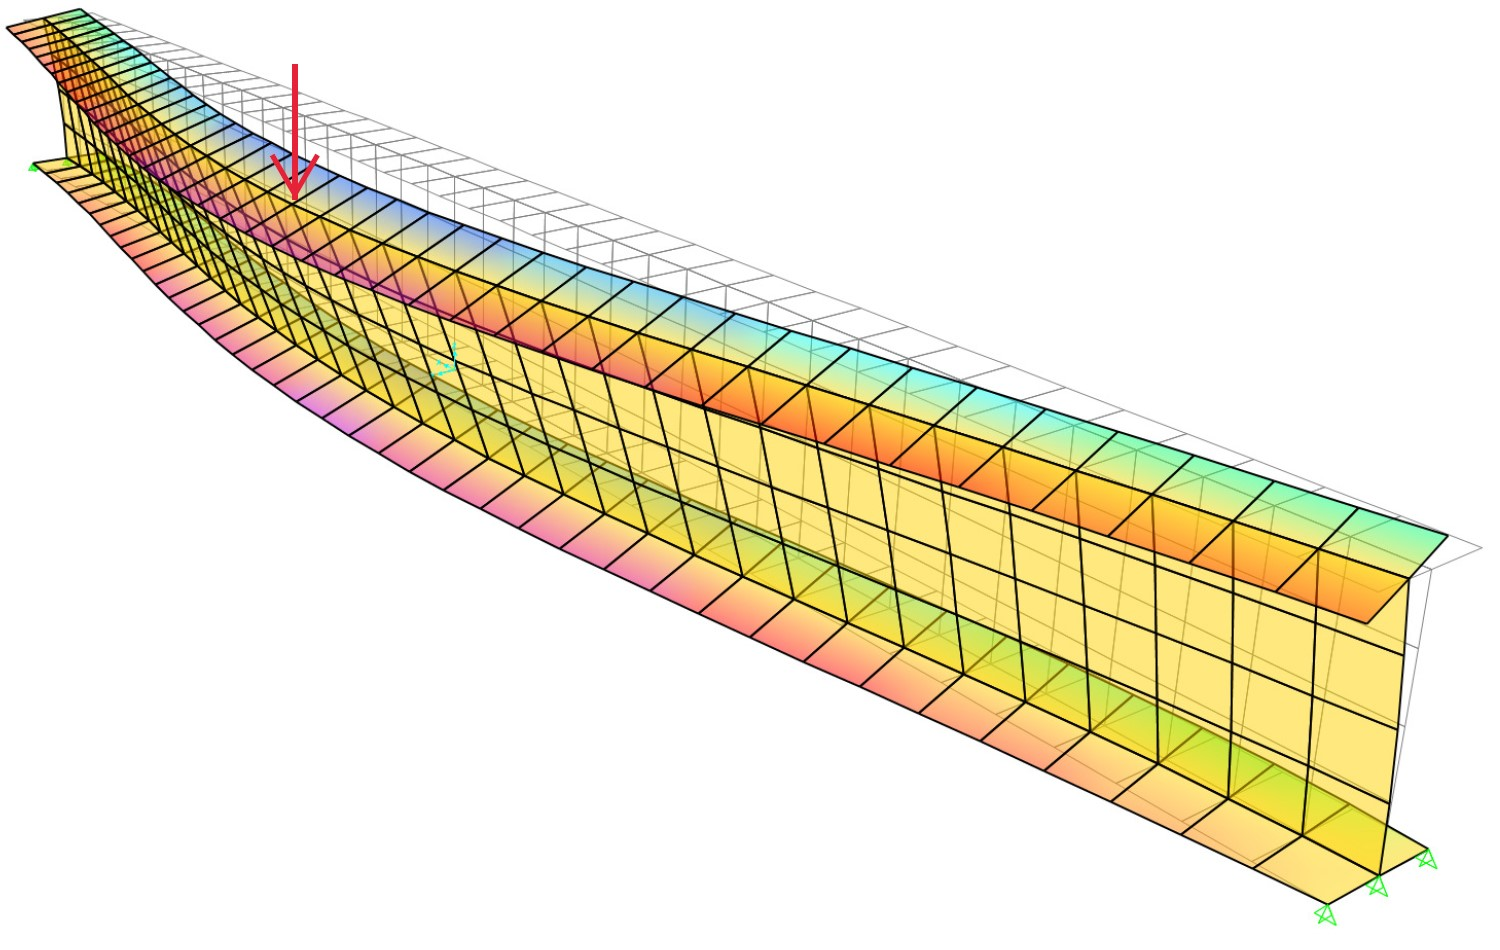
\includegraphics[width=0.45\textwidth]{PandeoViga}
	\label{fig:PandeoViga}}
\caption{Sistemas estructurales continuos}
	\label{fig:PandeoContinuo}
\end{figure}

El problema de minimización de la energía potencial total en el caso de $\bfu$ continua escapa de las herramientas usuales de Cálculo Vectorial y cae dentro del campo de Cálculo Variacional. En este curso no se presentará un tratamiento formal de esta última rama del cálculo, pero si se deducirán algunos resultados puntuales usando ideas asociadas al mismo.

Por otro lado, en el caso de estructuras discretas, la configuración deformada de la estructura $\bfu$ puede ser expresada mediante un número $n\in\mathbb{N}$ de valores reales. En este caso se dice que la estructura tiene $n$ grados de libertad o que $\mcU$ es un espacio de dimensión finita.

En la \autoref{fig:PandeoDiscreto} se pueden ver algunos ejemplos de sistemas estructurales discretos.

\begin{figure}[htb]
	\centering
\subfloat[Resorte de giro]{
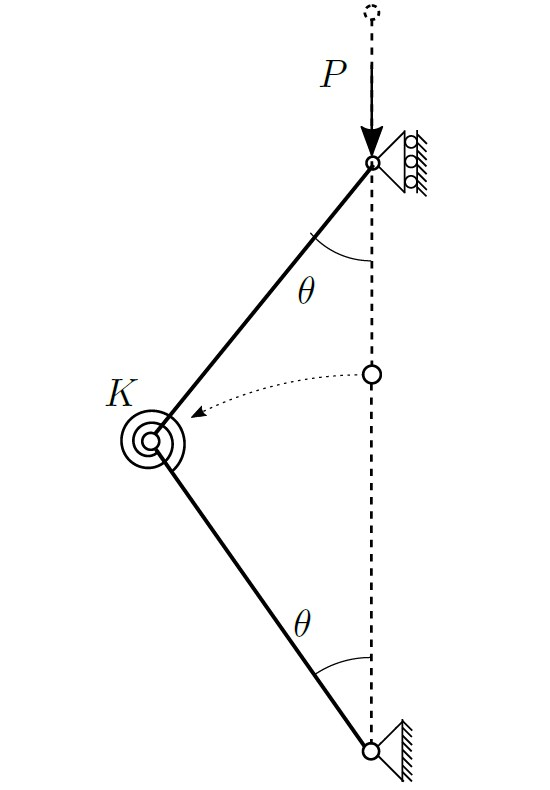
\includegraphics[width=0.25\textwidth]{Discreto1}
	\label{fig:Discreto1}}
\hspace{6em}
\subfloat[Resorte de desplazamiento]{
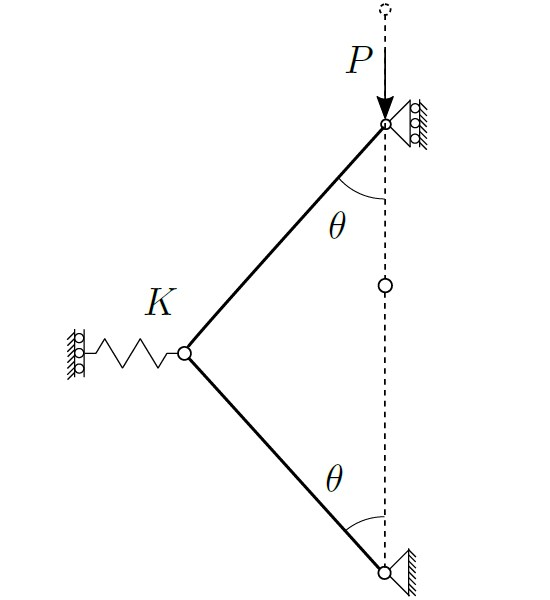
\includegraphics[width=0.3\textwidth]{Discreto2}
	\label{fig:Discreto2}}
\caption{Esquemas de sistemas estructurales discretos}
	\label{fig:PandeoDiscreto}
\end{figure}

Como se indicó en la sección anterior, el problema de minimización para el caso de estructuras discretas efectivamente puede resolverse con herramientas de Cálculo Vectorial usual, el planteo es particularmente sencillo si tenemos que $\Pi(\bfu)$ es suave. En ese caso, $\bfu \in \mathbb{R}^n$ es solución si se cumple que:
%
$$\nabla \Pi(\bfu)=0 \quad \text{y} \quad  \bfH_\Pi (\bfu), \text{es definida positiva},$$
%
donde $\bfH_\Pi(\bfu)$ es la matriz Hessiana de la función $\Pi(\bfu)$. Es decir, la matriz de derivadas parciales de grado dos respecto de $\bfu$ de la función $\Pi(\bfu)$.

%(0.5c) Presentar concepto de sistemas discretos y continuos. Ejemplos sin planteo ni solución (barras y resortes, vigas, placas)

\subsection{Equilibrio en Configuración Deformada}

Hasta aquí se ha presentado el criterio para determinar si un punto de equilibrio de una estructura es estable o no, pero no se ha descrito con detalle de qué manera debemos modificar las hipótesis del modelo estructural lineal de manera de poder evaluar correctamente la estabilidad elástica de una estructura.

El cambio fundamental de hipótesis necesaria para poder modelar la inestabilidad elástica en una estructura es pasar a considerar el equilibrio en la configuración deformada. Es decir que se deben considerar las fuerzas como actuando sobre la geometría deformada de la estructura.

En esta sección se presentan las condiciones de equilibrio para vigas considerando desplazamientos no despreciables. Se utiliza un desarrollo basado parcialmente en la Sección 1.6 de \citep{yoo2011}.

Si adicionalmente se desea tener modelos estructurales que permitan evaluar grandes rotaciones de elementos y grandes desplazamientos, entonces se deben incorporar expresiones exactas de la cinemática de la estructura. Un ejemplo típico de esto es la curvatura exacta de una viga, la cual en hipótesis de pequeños giros se simplifica por una derivada segunda de la deformación lateral de la viga.

En el marco del Principio de Mínima Energía Potencial Total, la capacidad de modelar la inestabilidad elástica se reduce a considerar correctamente el trabajo que hacen las fuerzas externas sobre la geometría deformada de la estructura.


\begin{figure}[htb]
	\centering
	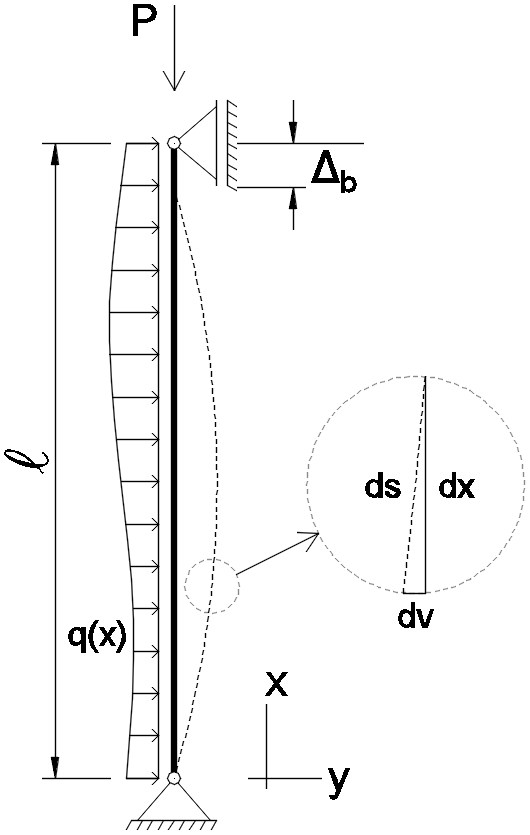
\includegraphics[width=0.3\textwidth]{confdef}
	\caption{Configuracion deformada de la columna.}
	\label{fig:confdef}
\end{figure}

A partir de la \autoref{fig:confdef} se considera la configuración de equilibrio de la columna con las cargas actuando sobre la configuración deformada. Se considera además que la columna se encuentra próxima al límite de bifurcación entre las distintas ramas de configuraciones de equilibrio.
Se recuerda que la energía potencial de deformación de la viga por flexión está dada por:
%
\begin{equation}
\Pi_{int} = \frac{1}{2} \int_\Omega \bfsig : \bfvarep  \dif V  = \frac{1}{2} \int_\Omega \sigma_x \varepsilon_x  \dif V. 
\end{equation}

Donde sustituyendo las Ecuaciones \eqref{eqn:eccons} y \eqref{eqn:expdef} y asumiendo que se desprecia la deformación axial $\varep_G$ previa al pandeo se tiene:
%
\begin{equation}
\Pi_{int} = \frac{1}{2} \int_0^\ell \int_{A(x)} E y^2 \left( \frac{\partial^2 v}{\partial x^2}\right)^2  \dif A \dif x 
=  E I  \frac{1}{2} \int_0^\ell \left( \frac{\partial^2 v}{\partial x^2}\right)^2 \dif x.
\end{equation}

En este caso se asumió que $EI$ es uniforme en la viga, un razonamiento análogo puede ser realizado sin esta hipótesis.

Para determinar la energía potencial, también se esta despreciando la contribución de las deformaciones por cortante debido a que estas son pequeñas respecto de las de flexión.

Se está usando que se desprecia la deformación axial previa al pandeo, por lo tanto el descenso vertical $\Delta_b$ debido a la flexión se puede escribir como:

\begin{equation}
\Delta_b = \ell - \int_{\mathscr{C}_d} dx = \ell - \int_{\mathscr{C}_d} \sqrt{ds^2-dv^2} = \ell - 
\int_{\mathscr{C}_d} \sqrt{1-\left(\frac{\partial v}{\partial s}\right)^2} \dif s
\end{equation}

Que se puede aproximar por:

\begin{equation}\label{eqn:deltab}
\Delta_b = \ell - \int_{\mathscr{C}_d} \left[1 - \frac{1}{2}\left(\frac{\partial v}{\partial s}\right)^2\right] \dif s = \frac{1}{2} \int_0^\ell \left(\frac{\partial v}{\partial x}\right)^2 \dif x
\end{equation}

Se tiene entonces que la energía potencial de las fuerzas $\Pi^{tr}_{ext}$ para la carga aplicada está dada por:
\begin{equation}
\Pi_{ext}^{tr} = -\frac{1}{2} P \int_0^\ell  \left(\frac{\partial v}{\partial x}\right)^2 \dif x
\end{equation}

Por otra parte, para la carga distribuida $q(x)$, se tiene que la energía potencial de las fuerzas $\Pi^{tr}_{ext}$ está dada por:
\begin{equation}
\Pi_{ext}^{tr} =
- \int_0^\ell q(x) v(x) \dif x
\end{equation}

Obteniendo que la expresión de la energía potencial total es,

\begin{equation}\label{eqn:energiatotal}
\Pi = E I \frac{1}{2} \int_0^\ell \left( \frac{\partial^2 v}{\partial x^2}\right)^2 \dif x -\frac{1}{2} P \int_0^\ell  \left(\frac{\partial v}{\partial x}\right)^2 \dif x - \int_0^\ell q(x) v(x) \dif x
\end{equation}

Se considera entonces una función arbitraria $\bar{v}(x)$ que solo satisface las condiciones de contorno y que cumple que $v(x)$ es la solución de deformación exacta buscada, de la siguiente manera,
\begin{equation}\label{eqn:funcionv}
\bar{v}(x)=v(x)+\varepsilon\eta(x)
\end{equation}
Donde se cumple que $\varepsilon$ es un número pequeño y $\eta(x)$ es una fúncion diferenciable con derivada segunda y que permite que $\bar{v}(x)$ satisfaga las condiciones geométricas de contorno, esto es que $\eta(0)=\eta(L)=0$.
La expresión anterior representa una pequeña perturbación arbitraria de la deformación de la columna respecto de la configuración de equilibrio y que se representa en la \autoref{fig:perturbacion}.

\begin{figure}[htb]
	\centering
	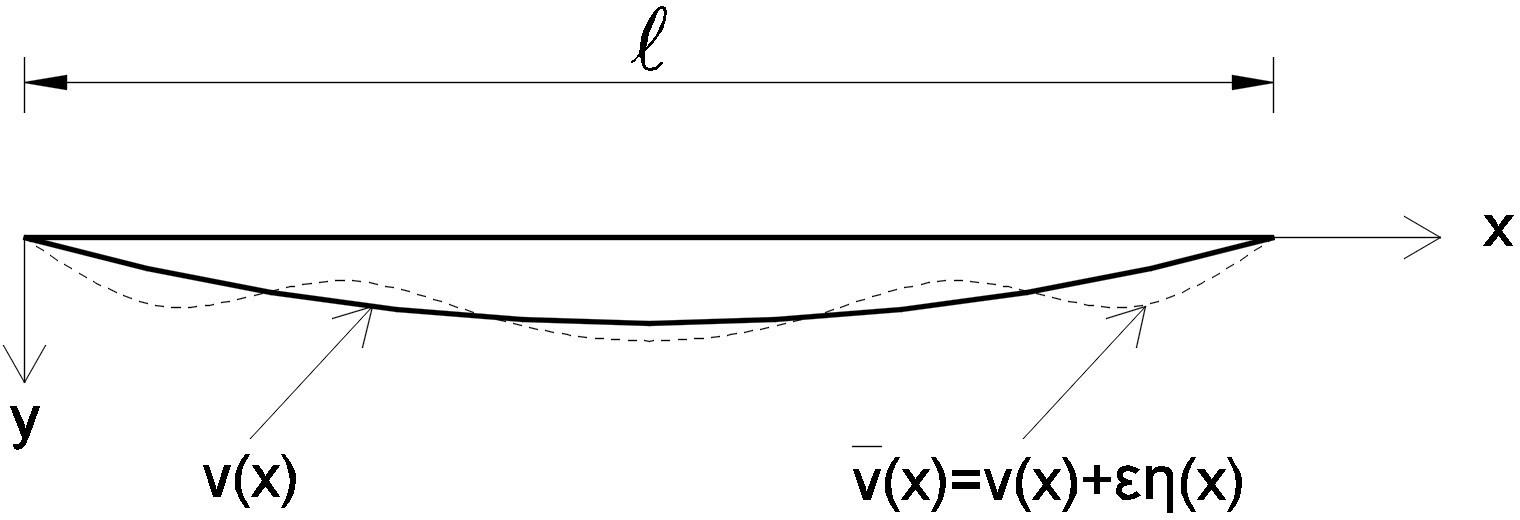
\includegraphics[width=0.5\textwidth]{perturbacion}
	\caption{Perturbación arbitraria de la deformación.}
	\label{fig:perturbacion}
\end{figure}

Si se sustituye la expresión \eqref{eqn:funcionv} en la Ecuación \eqref{eqn:energiatotal} se obtiene que la energía potencial para un desplazamiento arbitrario $\bar{v}(x)$ es

\begin{equation}\label{eqn:energiatotal2}
\Pi = \int_0^\ell \left[ \frac{EI}{2} \left( \frac{\partial^2 v}{\partial x^2} + \varepsilon\frac{\partial^2 \eta}{\partial x^2} \right)^2 - \frac{P}{2} \left(\frac{\partial v}{\partial x} + \varepsilon\frac{\partial \eta}{\partial x}\right)^2- q(x) \left( v(x)+\varepsilon\eta(x)\right) \right] \dif x
\end{equation}

La condición de Energía Potencial Interna estacionaria en $v(x)$ es igual a requerir que para todo $\eta(x)$ admisible, se debe de satisfacer que,

\begin{equation}
\frac{d\Pi}{d\varepsilon} \Bigg|_{\varepsilon=0} = 0
\end{equation}

A partir de la Ecuación \eqref{eqn:energiatotal2} se obtiene,
\begin{equation}
\frac{d\Pi}{d\varepsilon} = \int_0^\ell \left[ EI \left( \frac{\partial^2 v}{\partial x^2} + \varepsilon\frac{\partial^2 \eta}{\partial x^2} \right) \frac{\partial^2 \eta}{\partial x^2} - P \left(\frac{\partial v}{\partial x} + \varepsilon\frac{\partial \eta}{\partial x}\right)\frac{\partial \eta}{\partial x}- q(x) \eta(x) \right] \dif x
\end{equation}

Obteniendo que para $\varepsilon=0$,
\begin{equation}\label{eqn:difenergia}
\frac{d\Pi}{d\varepsilon} \Bigg|_{\varepsilon=0} = \int_0^\ell \left[ EI \frac{\partial^2 v}{\partial x^2} \frac{\partial^2 \eta}{\partial x^2} - P \frac{\partial v}{\partial x}\frac{\partial \eta}{\partial x}- q(x) \eta(x) \right] \dif x = 0
\end{equation}

Para simplificar la Ecuación \eqref{eqn:difenergia} se aplican integración por partes y las condiciones de contorno $\eta(0)=\eta(\ell)=0$. Se tiene entonces que para el segundo término de la Ecuación \eqref{eqn:difenergia},

\begin{equation}\label{eqn:partes1}
\int_0^\ell \frac{\partial v}{\partial x} \frac{\partial \eta}{\partial x}\dif x = \frac{\partial v}{\partial x}\eta\Bigg|_0^\ell - \int_0^\ell \frac{\partial^2 v}{\partial x^2} \eta\dif x 
= -\int_0^\ell \frac{\partial^2 v}{\partial x^2} \eta\dif x
\end{equation}

Por otra parte para el primer término de la Ecuación \eqref{eqn:difenergia} se tiene que,
$$
\int_0^\ell \frac{\partial^2 v}{\partial x^2} \frac{\partial^2 \eta}{\partial x^2}\dif x = \frac{\partial^2 v}{\partial x^2} \frac{\partial \eta}{\partial x}\Bigg|_0^\ell - \int_0^\ell \frac{\partial^3 v}{\partial x^3} \frac{\partial \eta}{\partial x}\dif x = \frac{\partial^2 v}{\partial x^2} \frac{\partial \eta}{\partial x}\Bigg|_0^\ell - \frac{\partial^3 v}{\partial x^3}\eta\Bigg|_0^\ell + \int_0^\ell \frac{\partial^4 v}{\partial x^4} \eta\dif x
$$

Obteniendo que,
\begin{equation}\label{eqn:partes2}
\int_0^\ell \frac{\partial^2 v}{\partial x^2} \frac{\partial^2 \eta}{\partial x^2}\dif x = \frac{\partial^2 v}{\partial x^2} \frac{\partial \eta}{\partial x}\Bigg|_0^\ell + \int_0^\ell \frac{\partial^4 v}{\partial x^4} \eta \dif x
\end{equation}

Sustituyendo las Ecuaciones \eqref{eqn:partes1} y \eqref{eqn:partes1} en la Ecuación \eqref{eqn:difenergia} se obtiene,

\begin{equation}\label{eqn:difenergia2}
\frac{d\Pi}{d\varepsilon} \Bigg|_{\varepsilon=0} = \int_0^\ell \left[ EI \frac{\partial^4 v}{\partial x^4} + P \frac{\partial^2 v}{\partial^2 x} - q(x)  \right] \eta(x) \dif x + EI\frac{\partial^2 v}{\partial x^2} \frac{\partial \eta}{\partial x}\Bigg|_0^\ell = 0
\end{equation}

Recordar que se debe cumplir para todo $\eta(x)$ admisible. Entonces en general se cumple además que, 

$$
\eta(x)\neq0 
\qquad
\frac{\partial \eta(0)}{\partial x} \neq 0
\qquad
\frac{\partial \eta(\ell)}{\partial x} \neq 0
\qquad 
\frac{\partial \eta(0)}{\partial x} \neq \frac{\partial \eta(\ell)}{\partial x}
$$

Por lo que para que la Ecuación \eqref{eqn:difenergia2} se cumpla se deben anular en simultáneo las siguientes:
\begin{eqnarray}
EI \frac{\partial^4 v}{\partial x^4}(x) + P \frac{\partial^2 v}{\partial^2 x}(x) - q(x) = 0 \qquad \text{Ecuación Euler-Lagrange} \label{eqn:euler} \\
EI\frac{\partial^2 v}{\partial x^2}\Bigg|_{x=0}=0 \qquad \text{Condición de contorno} \label{eqn:contorno1} \\
EI\frac{\partial^2 v}{\partial x^2}\Bigg|_{x=\ell}=0 \qquad \text{Condición de contorno} \label{eqn:contorno2}
\end{eqnarray}

Si bien las condiciones de contorno se impusieron al principio, se puede mostrar que estas condiciones no son estrictamente necesarias y que se puede obtener la misma ecuación diferencial que gobierna el problema \eqref{eqn:euler} para otras condiciones de contorno.

Por otra parte resulta de interés recordar la Ecuación \eqref{eqn:eqcortante} que aplicada en la Ecuación \eqref{eqn:euler} lleva a,
\begin{equation}\label{eqn:condcortante}
EI \frac{\partial^3 v}{\partial x^3}(x) + P \frac{\partial v}{\partial x}(x) - V(x) = 0
\end{equation}

También se recuerda la Ecuación \eqref{eqn:momen},  
\begin{equation}\label{eqn:condmomento}
M_z (x) = E I \frac{\partial^2 v}{\partial x^2}(x)
\end{equation}

\subsection{Solución Ecuación Homogénea}

La Ecuación \eqref{eqn:euler} es una ecuación de cuarto orden, lineal con un término independiente $q(x)$. Su solución estará compuesta por dos términos,
\begin{equation}
v(x)= v_p(x) + v_h(x)
\end{equation}

Donde $v_p(x)$ será una solución particular que dependerá de la carga distribuida $q(x)$ y $v_h(x)$ será la solución de la ecuación homogénea, esto es la solución de la ecuación diferencial cuando $q(x)=0$.

Se define,
\begin{equation}\label{eqn:defk}
k^2=\frac{P}{EI}
\end{equation}

De esta manera la Ecuación \eqref{eqn:euler} se puede reescribir como,
\begin{equation}\label{eqn:ecuahom}
\frac{\partial^4 v}{\partial x^4}(x) + k^2 \frac{\partial^2 v}{\partial^2 x}(x) = 0
\end{equation}

Utilizando un cambio de variable $\hat{v}=\frac{\partial^2 v}{\partial x^2}$ y sustityendo en la Ecuación~\eqref{eqn:ecuahom} se tiene
$$
\frac{\partial^2 \hat{v}}{\partial x^2}(x) + k^2 \hat{v}(x) = 0
$$
por lo que la solución homogénea sería
$$
\hat{v}(x) = \hat{A} \cos (kx) + \hat{B} \sin (kx).
$$

Volviendo atrás el cambio de variable, es decir, integrando esta solución se tiene la expresión de la solución de la ecuación homogénea $v$:
%
\begin{equation}
v(x) = A \cos (kx) + B \sin (kx) + Cx + D
\end{equation}
%
donde las constantes multiplicando $\cos$ y $\sin$ fueron renombradas y las constantes $A$, $B$, $C$ y $D$ deben determinarse empleando las condiciones de contorno sobre la solución particular en cada problema como se verá en la Sección~\ref{sec:componentes}.


\subsection{Puntos Críticos}

En esta sección se presenta una clasificación de puntos críticos a través de un conjunto de sistemas estructurales formados por barras rígidas unidas por articulaciones y resortes elásticos lineales (de desplazamiento y/o de giro). Para cada estructura y sistema de cargas se muestran las curvas de carga-desplazamiento para la estructura sin imperfecciones (curva que parte del origen en color negro) y con imperfecciones geométricas (curvas que presentan un desplazamiento para carga nula en color azul). Los tramos de trazo continuo representan equilibrios estables mientras que los tramos discontinuos puntos de algún tipo de inestabilidad.

\subsubsection{Bifurcación Simétrica Estable}

Una bifurcación simétrica estable corresponde a una situación en la cual una estructura alcanza un punto crítico y a partir de ese punto, su curva de carga-desplazamiento se bifurca en varias ramas: una inestable y otras dos estables.

El pandeo de columnas elásticas pertenece a esta categoría. En la Figura\autoref{fig:discreto11} se puede ver una versión discreta de ese tipo de estructura. En estos casos, al alcanzarse la bifurcación las estructuras logran mantener la carga aunque sea con grandes deformaciones (ej. columna elástica en compresión). En la Figura\autoref{fig:critico1} se muestra la curva carga-desplazamiento correspondiente. Notar que estas estructuras no son sensibles a imperfecciones, siempre y cuando el comportamiento material permanezca elástico.
\begin{figure}[htb]
	\centering
\subfloat[Esquema de estructura]{
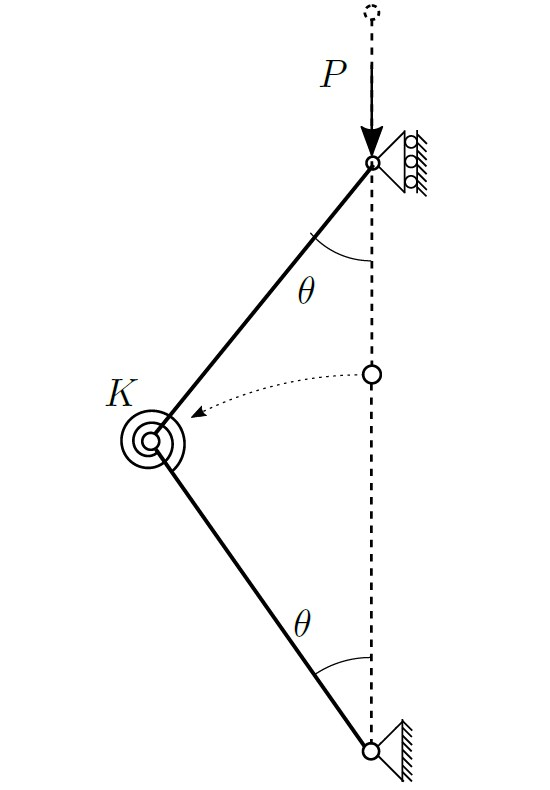
\includegraphics[width=0.25\textwidth]{Discreto1}
	\label{fig:discreto11}}
\hspace{1em}
\subfloat[Curva carga-desplazamiento]{
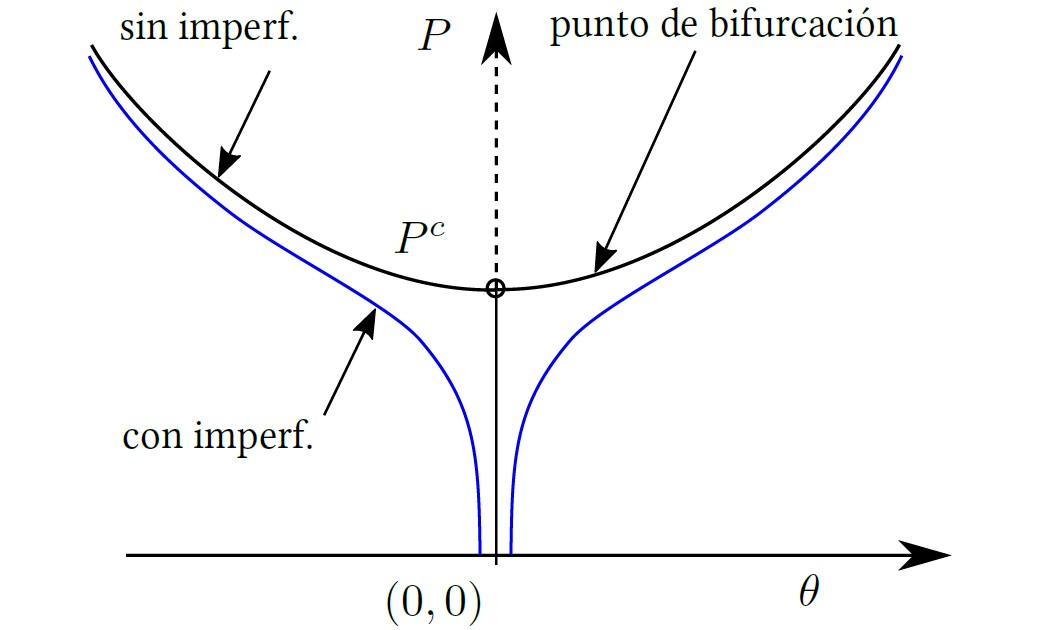
\includegraphics[width=0.55\textwidth]{Puntocritico1}
	\label{fig:critico1}}
\caption{Estructura con comportamiento de bifurcación simétrica estable}
	\label{fig:simetrica1}
\end{figure}

\subsubsection{Bifurcación Simétrica Inestable}

Este tipo de comportamiento se corresponde al de estructuras y cargas tales que, al alcanzarse la carga crítica, la curva de carga-desplazamiento se divide en varias ramas, todas inestables. La rama inicial (fundamental) es la única estable.

Las cáscaras esbeltas sometidas a compresión muestran este tipo de inestabilidad, ya que al alcanzar el punto de bifurcación pierden la capacidad de soportar la carga (ej. lata de aluminio en compresión). En la Figura\autoref{fig:discreto21} se muestra una estructura discreta que exhibe este comportamiento, la configuración de la estructura sin carga aplicada es representada por líneas punteada $(\theta = 0)$ mientras que en líneas sólidas se muestra la configuración deformada.

En el gráfico de la Figura\autoref{fig:critico2} se observa que el comportamiento de estas estructuras es considerablemente sensible a imperfecciones. En general, la carga máxima soportada por la estructura decrece al considerar imperfecciones geométricas. El resultado observado en este ejemplo pone en evidencia la importancia de este tipo de análisis en estructuras como cáscaras.
\begin{figure}[htb]
	\centering
\subfloat[Esquema de estructura]{
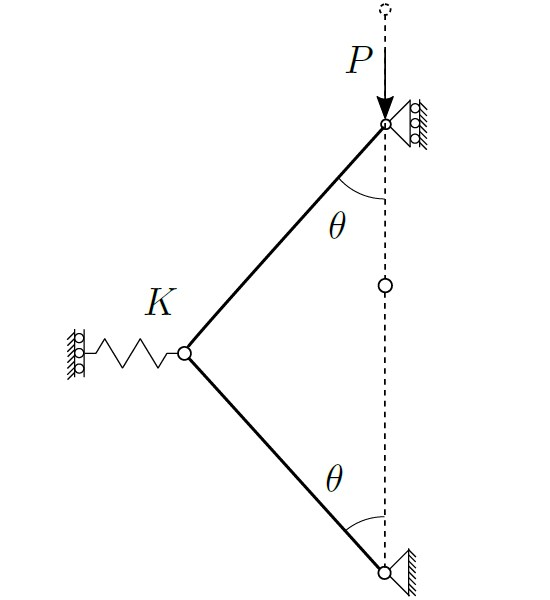
\includegraphics[width=0.3\textwidth]{Discreto2}
	\label{fig:discreto21}}
\hspace{1em}
\subfloat[Curva carga-desplazamiento]{
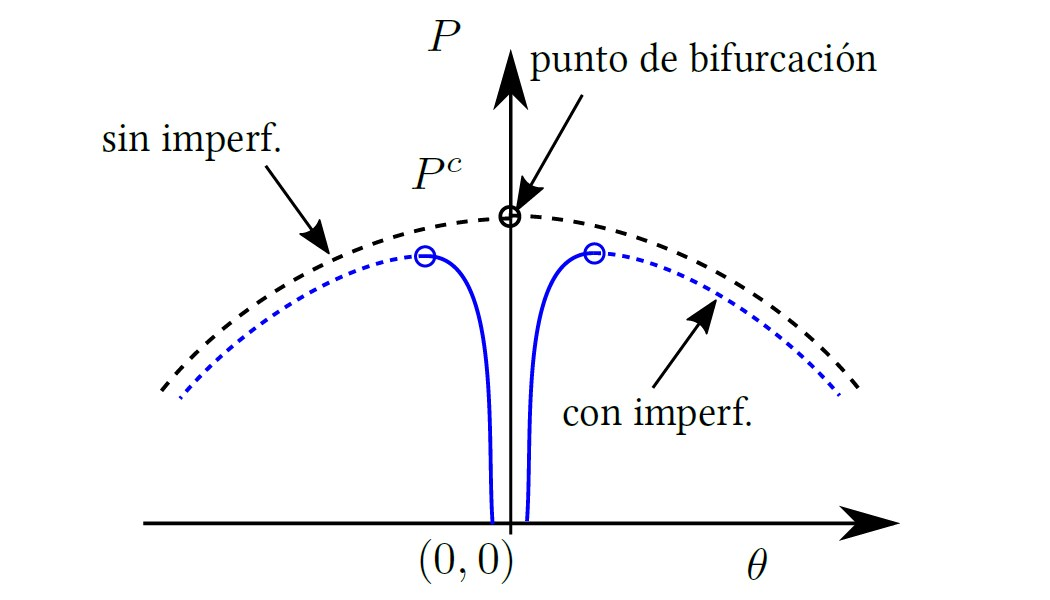
\includegraphics[width=0.55\textwidth]{Puntocritico2}
	\label{fig:critico2}}
\caption{Estructura con comportamiento de bifurcación simétrica inestable}
	\label{fig:simetrica2}
\end{figure}

\subsubsection{Bifurcación Asimétrica}

Este tipo de comportamiento corresponde a situaciones en las cuales la estructura alcanza una configuración de equilibrio inestable en la cual la curva de carga-desplazamiento se divide en varias ramas: dos ramas inestables y una estable. En la
Figura\autoref{fig:discreto31} se muestra otro ejemplo de estructura con este comportamiento. En la Figura\autoref{fig:critico3} se muestran las curvas de carga-desplazamiento.

Considerando perturbaciones o imperfecciones hacia un lado la estructura se sigue una rama estable, mientras que con perturbaciones hacia el otro lado se sigue una rama inestable, con lo cual, se clasifica como inestable en general. Consecuentemente la estructura es considerada como sensible a imperfecciones.
\begin{figure}[htb]
	\centering
\subfloat[Esquema de estructura]{
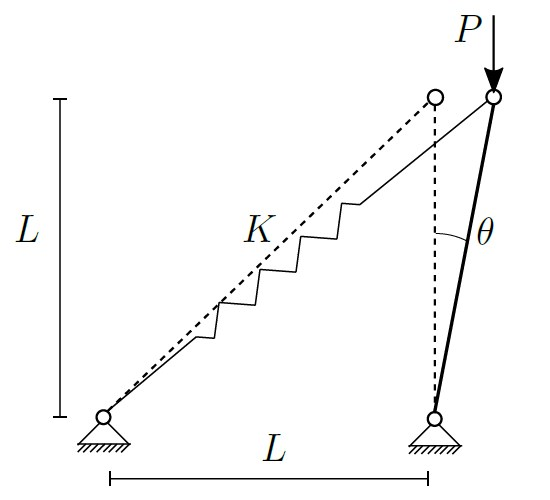
\includegraphics[width=0.3\textwidth]{Discreto3}
	\label{fig:discreto31}}
\hspace{1em}
\subfloat[Curva carga-desplazamiento]{
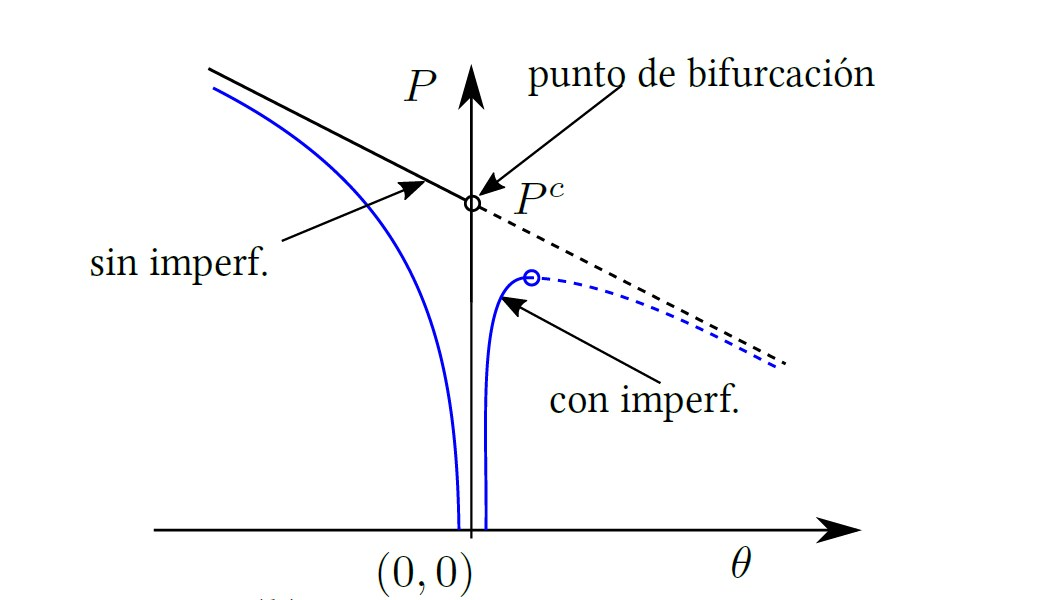
\includegraphics[width=0.55\textwidth]{Puntocritico3}
	\label{fig:critico3}}
\caption{Estructura con comportamiento de bifurcación asimétrica}
	\label{fig:asimetrica}
\end{figure}


\section{Estabilidad Elástica de Componentes} \label{sec:componentes}

\subsection{Columna de Euler}


\begin{figure}[htb]
	\centering
	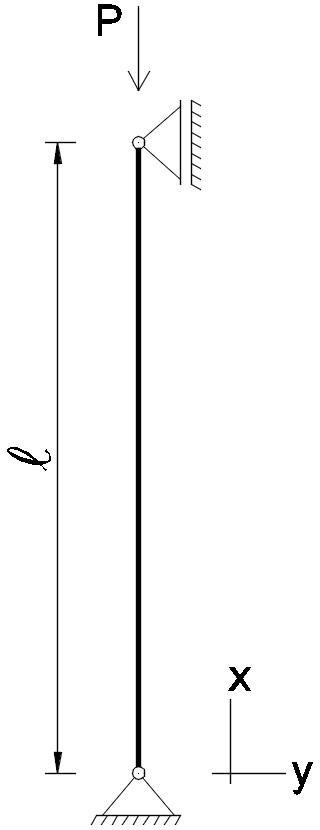
\includegraphics[width=0.15\textwidth]{euler}
	\caption{Columna de Euler.}
	\label{fig:euler}
\end{figure}

La ecuación diferencial de la deflexión $v$ está dada por la Ecuación \eqref{eqn:euler} y la solución y sus derivadas están dadas por:
\begin{eqnarray}
v(x) &=& A \cos(k x ) + B \sin(kx) + C x + D, \\
\frac{\partial   v}{\partial x  } (x) &=& -A k \sin(k x ) + B k \cos(kx) + C , \\
\frac{\partial^2 v}{\partial x^2} (x) &=& - A k^2 \cos(k x ) - B k^2 \sin(kx)
\end{eqnarray}
con k según la Ecuación \eqref{eqn:defk}

Las condiciones de contorno en función de las flechas o solicitaciones son,
\begin{equation}
\left\{
\begin{array}{l}
v(0)=0 \\[.5em]
\displaystyle v(\ell)=0\\[1em]
M(0)=0\\[.5em]
M(\ell)=0
\end{array}
\right.
\end{equation}

Aplicando las condicions anteriores tenemos
\begin{eqnarray}
v(0) &=& 0 \Rightarrow A + D = 0, \\
v(\ell) &=& 0 \Rightarrow A \cos(k \ell) + B \sin(k \ell) + C \ell + D = 0, \\
M(0) &=& EI \frac {\partial^2 v}{\partial x^2} (0) = 0 \Rightarrow -Ak^2 = 0,  \\
M(\ell) &=& EI \frac{\partial^2 v}{\partial x^2} (\ell) = 0  \Rightarrow -Ak^2\cos(k \ell) -  B k^2 \sin(k\ell) = 0,
\end{eqnarray}

De las ecuaciones anteriores y teniendo en cuenta que $k>0$ se obtiene que se deben cumplir las siguientes condiciones
\begin{equation}
A = B\sin(k\ell) = C = D = 0
\end{equation}

Por lo tanto existen dos alternativas, $A = B = C = D = 0$, que es la solución trivial ya conocida o que $\sin(k\ell) = 0$.
Para que esto último se cumpla se tiene que,
\begin{equation}
k \ell = n \pi  \quad \text{con} \,\, n\in \bbN
\end{equation}

En ese caso cualquier valor de $B$ cumple la condición por lo que existen infinitas soluciones. En particular la menor directa asociada a estos valores de $k$ es con $n=1$,
\begin{equation}\label{eqn:criticaeuler}
\boxed{P_{cr} = \frac{\pi^2 E I}{\ell^2}}
\end{equation}
Siendo esta la expresión de la Carga Crítica que produce la inestabilidad en la Columna de Euler.

\subsection{Luz de Pandeo}

Se considera $\ell$ como la luz libre del elemento en estudio, se define entonces $L_P$ como la luz de pandeo de dicho elemento, como
\begin{equation}
L_P=\beta\ell
\end{equation}
Donde $\beta$ depende de los vínculos que tenga el elemento. De esta manera la expresión de Carga Crítica \eqref{eqn:criticaeuler} se puede generalizar como,
\begin{equation}\label{eqn:criticageneral}
\boxed{P_{cr} = \frac{\pi^2 E I}{L_P^2}}
\end{equation}

Para un elemento simplemente apoyado se determinó que la Carga Crítica es,
$$P_{cr} = \frac{\pi^2 E I}{\ell^2}$$
mientras que para un elemento en ménsula, con un extremo empotrado y otro libre, se verá mas adelante que la Carga Crítica es,
$$P_{cr} = \frac{\pi^2 E I}{4\ell^2}$$
Se observa que para el caso del elemento simplemente apoyado la luz de pandeo es $L_P=\ell$ y por lo tanto $\beta=1$, mientras que para el caso del elemento en ménsula la luz de pandeo es $L_P=2\ell$ y por lo tanto $\beta=2$. 

Se puede observar en la Figura~\ref{fig:luzpandeo} que el caso del elemento en ménsula puede ser asimilado al caso de un elemento simplemente apoyado de longitud $2\ell$. Resolviendo analíticamente otros casos y realizando un razonamiento similar se puede ver que la luz de pandeo es también la distancia entre dos puntos de momento nulo. Esto último implica que la longitud de pandeo también se puede interpretar como aquella que separa puntos con curvatura acotada, debido a que los puntos de momento nulo coinciden con los puntos de inflexión de la elástica.

\begin{figure}[htb]
	\centering
	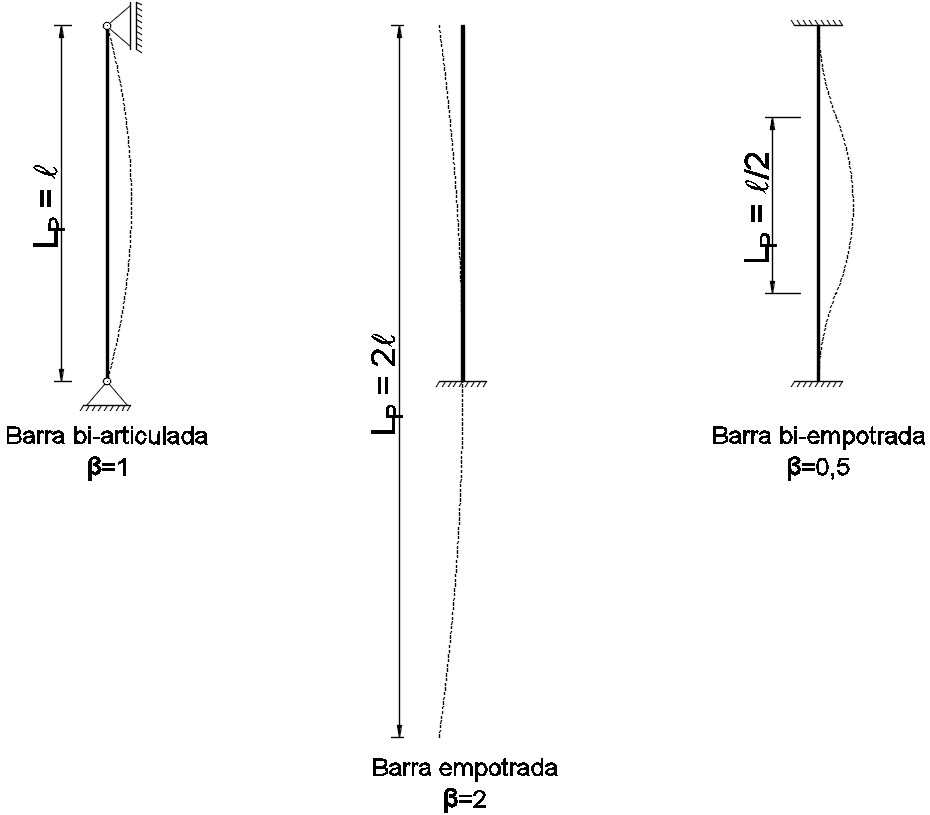
\includegraphics[width=0.6\textwidth]{LuzPandeo}
	\caption{Luz de Pandeo según condiciones de apoyo.}
	\label{fig:luzpandeo}
\end{figure}

\subsection{Esbeltez}

Se define la esbeltez $\lambda$ de un elemento comprimido de la siguiente manera,
\begin{equation}
\lambda = \frac{L_P}{\rho}
\end{equation}

Donde el radio de giro $\rho$ de la sección respecto de un eje principal cumple que
\begin{equation}
\rho^2 = \frac{I}{A}
\end{equation}

Si se sustituye en la Ecución \eqref{eqn:criticageneral} se tiene
$$
P_{cr} = \frac{\pi^2 E A \rho^2}{L_P^2} = \frac{\pi^2 E A}{\left(\frac{L_P}{\rho}\right)^2}
$$

Obteniendo que,
\begin{equation}
\boxed{P_{cr} = \frac{\pi^2 E A}{\lambda^2}}
\end{equation}

De igual manera y usando que $\sigma=P/A$ se puede definir una tensión de compresión crítica como  
\begin{equation}
\boxed{\sigma_{cr} = \frac{\pi^2 E}{\lambda^2}}
\end{equation}
Cuyo valor tiene como cota superior la tensión admisible $\sigma_{adm}$ del material.

Hasta ahora se ha estudiado el fenómeno de pandeo con propiedades geométricas $I$ y $\rho$ genéricas. Sin embargo, si los vínculos del elemento son iguales en ambas direcciones la carga crítica quedará determinada por el menor momento de inercia. Por otra parte, para analizar el fenómeno de pandeo en elementos con vínculos distintos en cada dirección, será necesario estudiar ambas direcciones por separado con el momento de inercia que corresponda, quedando en general determinado por la dirección de mayor esbeltez.

\subsection{Ejemplo: ménsula con carga axial}

Se considera una ménsula formada por un material de módulo de Young $E$, de largo $\ell$ con sección transversal de inercia $I$ sometida a una carga axial de compresión $N=P$ aplicada en su extremo libre con una excentricidad $e$, como se muestra en la Figura~\ref{fig:esqpand}. %
%
No hay carga transversal aplicada, por lo tanto $q=0$. %

\begin{figure}[htb]
\centering
\def\svgwidth{0.5\textwidth}
\input{figs/UT7/ejemplo_pandeo.pdf_tex}
\caption{Esquema de ménsula con carga axial con excentricidad.}
\label{fig:esqpand}
\end{figure}

En estructuras reales, excentricidades como la considerada pueden ser provocadas por errores en la ejecución de elementos estructurales conectados a la ménsula (por ejemplo vigas descargando sobre columnas). %
%
Esto permite considerar la excentricidad como una \textit{imperfección}, la cual usualmente tiene magnitud considerablemente menor a las dimensiones de la sección transversal. %
% ------------------------------------------

Como ya se vió, la ecuación diferencial de la deflexión $v$ está dada por la Ecuación \eqref{eqn:euler}
$$
  E I \frac{\partial^4 v}{\partial x^4}(x)
+   P \frac{\partial^2 v}{\partial x^2}(x)
=   0
$$

La solución y sus derivadas están dadas por:
\begin{eqnarray}
v(x) &=& A \cos(k x ) + B \sin(kx) + C x + D, \\
\frac{\partial   v}{\partial x  } (x) &=& -A k \sin(k x ) + B k \cos(kx) + C , \\
\frac{\partial^2 v}{\partial x^2} (x) &=& - A k^2 \cos(k x ) - B k^2 \sin(kx),  \\
\frac{\partial^3 v}{\partial x^3} (x) &=& A k^3 \sin(k x ) - B k^3 \cos(kx), 
\end{eqnarray}
con k según la Ecuación \eqref{eqn:defk}

Las condiciones de contorno en función de las flechas o solicitaciones son,
\begin{equation}
\left\{
\begin{array}{l}
v(0)=0 \\[.5em]
\displaystyle \frac{\partial v}{\partial x}(0)=0\\[1em]
V(\ell)=0\\[.5em]
M(\ell)=-P e
\end{array}
\right.
\end{equation}

Es necesario obtener las condiciones de contorno en función de la flecha. %
Se comienza desarrollando la condición del cortante, es decir,
%
\begin{equation}
	V(\ell) = 0,
\end{equation}
Utilizando la Ecuación \eqref{eqn:condcortante} y operando se obtiene la relación equivalente, en función de la flecha:
%
\begin{equation}
  \frac{\partial^3 v}{\partial x^3} (\ell) = - k^2 \frac{\partial v}{\partial x}(\ell).
\end{equation}
%
Sustituyendo la expresión de la solución se tiene:
%	
\begin{equation}
	Ak^3 \sin(k\ell) - Bk^3 \cos(k\ell) = Ak^3 \sin(k\ell) - Bk^3 \cos(k\ell) - C k^2,
\end{equation}
por lo tanto se cumple:
\begin{equation}\label{eqn:ejemplopand}
\boxed{
  C=0
}
\end{equation}

Usando la condición de giro nulo en el empotramiento se tiene
\begin{equation}
v'(0)=0 \Leftrightarrow  Bk + C = 0,
\end{equation}
%
por lo tanto usando la Ecuación~\eqref{eqn:ejemplopand} se tiene
\begin{equation}
\boxed{
B=0
}
\end{equation}

Usando la Ecuación \eqref{eqn:condmomento} y la condición de momento en $\ell$ se tiene
%
\begin{equation}
M(\ell) = -P e \Leftrightarrow \frac{\partial v^2}{\partial x^2} (\ell)  = - k^2 e
\end{equation}
%
por lo tanto
%
\begin{equation}
-k^2 A \cos(k\ell) - k^2 B \cos(k\ell) = -k^2 e
\end{equation}

Esto es equivalente a 
\begin{equation}\label{eqn:acos}
\boxed{
A \cos(k\ell)  = e
}
\end{equation}

Finalmente usando la condición de desplazamiento nulo en el empotramiento se tiene
%
\begin{equation}
v(0)=0  \Leftrightarrow \boxed{ A + D = 0}
\end{equation}

Es necesario estudiar de forma independiente las soluciones obtenidas para los casos con y sin imperfecciones.

\subsubsection{Solución sin imperfección}

El caso sin imperfección corresponde a $e=0$ y la expresión solución está dada por:
%
\begin{equation}
v(x) = A (\cos(k x) -1), \quad \text{con} \quad A\cos(k\ell) = 0.
\end{equation}

Si se verifica
%
\begin{equation}
k \ell = \frac{\pi}{2} + n\pi  \quad \text{con} \,\, n\in \bbN,
\end{equation}
%
entonces cualquier valor de $A$ cumple la condición por lo que existen infinitas soluciones. %
%
En particular la menor directa asociada a estos valores de $k$ es
\begin{equation}
\boxed{
P_{cr} = \frac{\pi^2 E I}{4 \ell^2}}
\end{equation}
%
Esta carga crítica corresponde a una luz de pandeo $L_p = 2\ell$.

\subsubsection{Solución con imperfección}

En este caso se considera una excentricidad $e \neq 0$, por lo que se obtiene una única solución dada por:
%
\begin{equation}
v(x) = \frac{e}{\cos(k\ell)} (\cos(k x) -1).
\end{equation}
%
Se destaca que se asumió que $\cos(k \ell) \neq 0$, en caso contrario se tendría una incompatibilidad en la Ecuación~\eqref{eqn:acos}. %

Se mostrará que, de acuerdo con el modelo considerado, existe un nivel de carga para el cual la estructura pierde capacidad de soportar cargas superiores (rigidez) y la flecha adquiere valores elevados. %
%

Como referencia se considera la flecha en el extremo libre, es decir:
%
\begin{equation}
v(\ell) = e \left( 1- \frac{1}{\cos(k\ell) }  \right)
\end{equation}
%
si $k=0$ se tiene un valor nulo de flecha, mientras que al aumentar el valor de $P$ se tiene un crecimiento que lleva a que cuando se alcanza el valor 
%
\begin{equation}
k = \frac{\pi}{2 \ell }
\end{equation}
%
la flecha tiende a infinito. %
%
Esto establece por lo tanto que la carga crítica de la estructura es la misma del caso anterior
%
\begin{equation}
\boxed{
	P_{cr} = \frac{\pi^2 E I}{4 \ell^2}.
}
\end{equation}


En la Figura~\ref{fig:ejpand} se presenta la curva de desplazamientos del extremo libre (abscisas) para diferentes valores de $k\ell$ (ordenadas). %
%
Para $k\ell$ se consideran 30 valores equiespaciados entre $0$ y $\frac{\pi}{2} 0.99$.

\begin{figure}[htb]
	\centering
		\resizebox{.7\textwidth}{!}{% Title: gl2ps_renderer figure
% Creator: GL2PS 1.3.9, (C) 1999-2015 C. Geuzaine
% For: Octave
% CreationDate: Mon Dec  4 08:08:25 2017
\setlength{\unitlength}{1pt}
\begin{picture}(0,0)
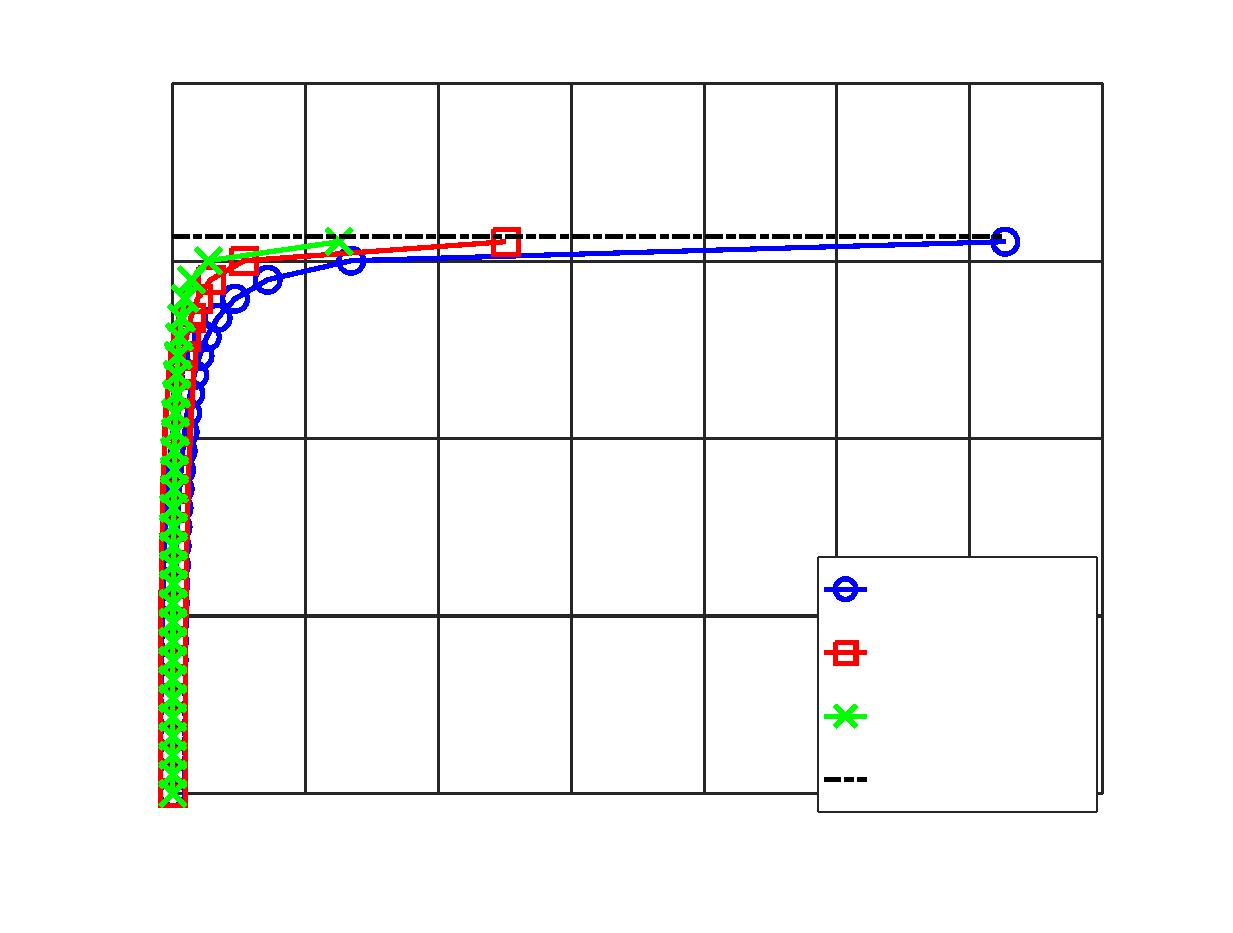
\includegraphics{plotejempand-inc}
\end{picture}%
\begin{picture}(576,432)(0,0)
\fontsize{22}{0}
\selectfont\put(74.88,54.0046){\makebox(0,0)[t]{\textcolor[rgb]{0.15,0.15,0.15}{{0}}}}
\fontsize{22}{0}
\selectfont\put(138.651,54.0046){\makebox(0,0)[t]{\textcolor[rgb]{0.15,0.15,0.15}{{5}}}}
\fontsize{22}{0}
\selectfont\put(202.423,54.0046){\makebox(0,0)[t]{\textcolor[rgb]{0.15,0.15,0.15}{{10}}}}
\fontsize{22}{0}
\selectfont\put(266.194,54.0046){\makebox(0,0)[t]{\textcolor[rgb]{0.15,0.15,0.15}{{15}}}}
\fontsize{22}{0}
\selectfont\put(329.966,54.0046){\makebox(0,0)[t]{\textcolor[rgb]{0.15,0.15,0.15}{{20}}}}
\fontsize{22}{0}
\selectfont\put(393.737,54.0046){\makebox(0,0)[t]{\textcolor[rgb]{0.15,0.15,0.15}{{25}}}}
\fontsize{22}{0}
\selectfont\put(457.509,54.0046){\makebox(0,0)[t]{\textcolor[rgb]{0.15,0.15,0.15}{{30}}}}
\fontsize{22}{0}
\selectfont\put(521.28,54.0046){\makebox(0,0)[t]{\textcolor[rgb]{0.15,0.15,0.15}{{35}}}}
\fontsize{22}{0}
\selectfont\put(69.8755,58.9987){\makebox(0,0)[r]{\textcolor[rgb]{0.15,0.15,0.15}{{0}}}}
\fontsize{22}{0}
\selectfont\put(69.8755,144.149){\makebox(0,0)[r]{\textcolor[rgb]{0.15,0.15,0.15}{{0.5}}}}
\fontsize{22}{0}
\selectfont\put(69.8755,229.299){\makebox(0,0)[r]{\textcolor[rgb]{0.15,0.15,0.15}{{1}}}}
\fontsize{22}{0}
\selectfont\put(69.8755,314.45){\makebox(0,0)[r]{\textcolor[rgb]{0.15,0.15,0.15}{{1.5}}}}
\fontsize{22}{0}
\selectfont\put(69.8755,399.6){\makebox(0,0)[r]{\textcolor[rgb]{0.15,0.15,0.15}{{2}}}}
\fontsize{22}{0}
\selectfont\put(298.08,27.0046){\makebox(0,0)[t]{\textcolor[rgb]{0.15,0.15,0.15}{{Desplazamiento $v(\ell)$}}}}
\fontsize{22}{0}
\selectfont\put(30.8755,229.299){\rotatebox{90}{\makebox(0,0)[b]{\textcolor[rgb]{0.15,0.15,0.15}{{$k \ell$}}}}}
\fontsize{22}{0}
\selectfont\put(410.88,157.064){\makebox(0,0)[l]{\textcolor[rgb]{0,0,0}{{$e=$ 0.5}}}}
\fontsize{22}{0}
\selectfont\put(410.88,126.549){\makebox(0,0)[l]{\textcolor[rgb]{0,0,0}{{$e=$ 0.2}}}}
\fontsize{22}{0}
\selectfont\put(410.88,96.0347){\makebox(0,0)[l]{\textcolor[rgb]{0,0,0}{{$e=$ 0.1}}}}
\fontsize{22}{0}
\selectfont\put(410.88,65.5203){\makebox(0,0)[l]{\textcolor[rgb]{0,0,0}{{$e=0$}}}}
\end{picture}
}
	\caption{Resultado analítico de inestabilidad con imperfección.}
	\label{fig:ejpand}
\end{figure}

Se puede observar cómo la presencia de imperfecciones de mayor magnitud provocan que la estructura tenga mayores desplazamientos para cada valor de carga dado. %
%
Para todas las excentricidades, la curva tiene una asíntota horizontal en $k\ell=\frac{\pi}{2}$, por lo que este modelo establece que la estructura no es capaz de soportar cargas superiores a la carga crítica.


La curvatura está dada por la función 
\begin{equation}
\frac{\partial^2 v}{\partial x^2}(x) = -k^2 e \frac{\cos(k x)}{\cos(k\ell)}.
\end{equation}


Se puede mostrar que
\begin{equation}
\lim\limits_{P\rightarrow P_{cr}}
\left| \frac{\partial^2 v}{\partial x^2}(x) \right|
 =
\left\{
\begin{array}{lr}
\infty & \text{si } x \in (-\ell,\ell)\\
\displaystyle \frac{\pi^2 e}{4 \ell^2} & \text{si } x \in \{-\ell,\ell\}
\end{array}
\right.
\end{equation}
%
por lo tanto, a partir de este resultado, se puede observar como la longitud de pandeo es aquella que separa puntos con curvatura acotada.


%\subsection{Otros Componentes}
% - (1c) Otros tipos de inestabilidad de componentes. Nombrar + Imagen (plot de Robot x ejemplo) y referir a Curso de Mecanica Estructural:
% * Inestabilidad torsional en columnas
% * Inestabilidad flexo-torsional en columnas
% * Inestabilidad lateral torsional en vigas

%\subsection{Inestabilidades Locales}
% - (1c) Inestabilidades en elementos de componentes referir a curso Estructuras de Acero:
% * Inestabilidad de alas y almas en compresión.
% * Inestabilidad de almas en corte.
% * Resistencia post-crítica de chapas planas permite tener capacidad más alla de carga crítica.


\section{Estabilidad global estructuras}
A continuación se hace una breve mención a la estabilidad global de estructuras. Hasta esta sección se presentaron conceptos de estabilidad que comprenden el comportamiento de componentes individuales. Dichos conceptos se pueden llevar al estudio de la estabilidad de ensamblajes de componentes, es decir la estabilidad de sistemas estructurales completos.

\subsection{Sistemas resistentes de esfuerzos laterales}
En el contexto de estructuras de edificación, se puede definir el concepto de sistema resistente de esfuerzos laterales como aquella parte de la estructura que tiene como función resistir las cargas laterales que puedan ser aplicadas sobre la estructura y llevar dichas cargas al suelo.

Un paso clave en la definición de la estructura de una edificación es identificar el sistema resistente de esfuerzos laterales. El mismo se puede componer de pantallas, núcleos o pórticos entre otros. No todas las columnas verticales tienen porqué integrar el sistema resistente de esfuerzos laterales; este puede ser el caso en la medida que dichas columnas no tengan la rigidez necesaria para tomar esfuerzos laterales o que las conexiones que las vinculan al resto de la estructura no permitan que participen de dicho sistema resistente.

\begin{figure}[htb]
  \centering
  %\width{0.6\textwidth}
%  \includegraphics[width=0.95\textwidth]{figs/UT7/Esquema_de_nucleos.png}
	\caption{Sistemas Resistentes de Esfuerzos Laterales. Izquierda: esquema en planta de planos resistentes. Derecha: Alzados de distintas opciones de planos resistentes.}
	\label{fig:EsqNucleos}
\end{figure}

Se deben definir sistemas resistentes de esfuerzos laterales de manera de poder soportar esfuerzos laterales en cualquier orientación y también esfuerzos laterales con excentricidades arbitrarias. Esto lleva a requerir para una estructura al menos tres planos verticales resistentes no concurrentes como mínimo. No obstante, basadándose en el criterio de robustez estructural, es decir que un fallo localizado en la estructura no genere un daño desproporcionado en la misma, se debería evitar tener una situación en la cual un fallo local saque de servicio a uno de los planos resistentes y la estructura pasa a tener una sistema resistente lateral insuficiente.


\subsection{Amplificación de Efectos Globales}

Las normas actuales de diseño de estructuras de tipo edificación tanto de hormigón como de acero requieren que se evalúen los efectos de segundo orden esperados cuando la estructura se esté aproximando a su máxima capacidad resistente. Esto incluye tanto los efectos de segundo orden a nivel de componentes (i.e. P-$\delta$), así como los efectos de segundo orden globales (i.e. P-$\Delta$).

A continuación presentamos un resumen del tipo de enfoque que se presenta en la norma europea para la amplificación de efectos globales en estructuras de tipo edificación de hormigón (i.e. EN 1992-1-1). Más precisamente, se justificarán algunas de las expresiones presentadas en el Anexo H de dicha norma.

Considere una estructura compuesta de un pórtico traslacional 2-D el cual arriostra una serie de columnas bi-articuladas. Esta estructura busca simular edificio de una planta, donde el pórtico actúa como sistema resistente lateral.

\begin{figure}[htb]
  \centering
  \def\svgwidth{0.8\textwidth}
  \input{figs/UT7/globales.pdf_tex}
	\caption{Estructura de pórtico traslacional arriostrando columnas.}
	\label{fig:globales}
\end{figure}

La estructura tiene cargas verticales gravitatorias y una cierta carga lateral que puede provenir por ejemplo del efecto del viento.

Se propone realizar un análisis simplificado y aproximado del comportamiento de la estructura. En dicho análisis, se cambia el pórtico traslacional por un resorte lateral con igual rigidez lateral ($K_{p}$) que dicho pórtico.

\begin{figure}[htb]
  \centering
  \def\svgwidth{0.6\textwidth}
  \input{figs/UT7/globales2.pdf_tex}
	\caption{Resorte equivalente a pórtico traslacional arriostrando columnas.}
	\label{fig:globales2}
\end{figure}

El único grado de libertad de la estructura pasa a ser el desplazamiento lateral del piso superior ($u$). Se puede, por lo tanto, expresar la energía potencial total como función de dicho grado de libertad.

Se debe observar que cuando los extremos superiores de las columnas se mueven $u$ hacia el costado, dichos extremos descienden una cantidad $w(u)=H-\sqrt{H^2-u^2}$. Este descenso puede ser aproximado a orden dos, Maclaurin de por medio, como $w(u)=u^2/(2H)$.

La energía potencial total resulta por lo tanto:

$$\Pi(u)=K_p \frac{u^2}{2} -\sum_{i=1}^n P_i w(u) - F_H u$$

Substituyendo el descenso $w(u)$ por su expresión aproximada en función de $u$ y notando que es igual para todos los puntos de aplicación de las cargas $P_i$:

$$\Pi(u)=K_p \frac{u^2}{2} -\frac {u^2}{2H} \sum_{i=1}^n P_i - F_H u$$

Podemos evaluar por lo tanto el equilibrio de la estructura estudiando la condición de $\nabla \Pi(u)=0$ y la estabilidad del sistema estudiando la derivada segunda de $\Pi(u)$ en los puntos de equilibrio.

$$\frac{d \Pi(u))}{d u} = \left(K_p-\frac{\sum_{i=1}^n P_i}{H}\right)u - F_H = 0$$

Se debe reconocer que si se hubiera analizado la estructura linealmente, el desplazamiento lateral de equilibrio hubiera sido igual a $u^{(0)}=F/K_p$.

En adelante se denominará la carga vertical total sobre la estructura como $P_{tot}=\sum_{i=1}^n P_i$. A partir de la ecuación anterior se deduce que el desplazamiento lateral aproximado de segundo orden es igual a:

$$u=\frac{F_H}{K_p - P_{tot}/H}$$

Se procede a evaluar la estabilidad de los equilibrios por medio del estudio de la derivada segunda de la energía potencial total:

$$\frac{d^2 \Pi(u))}{d u^2} = K_p-\frac{P_{tot}}{H}$$

El equilibrio se tornará crítico (i.e. la estructura pasará de ser estable a inestable) cuando dicha derivada segunda se anule:

$$\left.\frac{d^2 \Pi(u))}{d u^2}\right|_{cr} = K_p-\frac{P_{tot,cr}}{H}=0$$

De donde se deduce que la carga vertical total crítica es igual a:

$$P_{tot,cr} = K_p H$$

Usando esta expresión de carga crítica, se puede expresar la deformación lateral aproximada de segundo orden de la siguiente manera:

$$u=\frac{u^{(0)}}{1 - P_{tot}/P_{tot,cr}}$$

Es decir, el sistema resistente lateral se desplazará lateralemente más cuanto mayor sean las cargas verticales totales relativas a la carga vertical crítica total de la estructura.

La norma EN 1992-1-1 presenta en el anexo H las siguientes expresiones equivalentes a las deducidas en esta sección:

\begin{figure}[htb]
	\centering
	%\width{0.6\textwidth}
	AGREGAR FIGURA
%	\includegraphics[width=0.7\textwidth]{EN_Pcrit.png}
	\caption{EN 1992-1-1, Anexo H. Carga crítica Global para sistemas resistentes laterales con deformación lateral de tipo distorisión.}
	\label{fig:EN_Pcrit}
\end{figure}

Para poder reconocer la carga crítica dada el anexo G, se debe reconocer que $\Sigma S$, la fuerza lateral soportada por el pórtico dividida por el ángulo de distorsión lateral ($\gamma = u / H$) del pórtico, es igual a:

$$ \Sigma S = \frac{F_H}{\gamma} = \frac{K_p u}{u/H} = K_p H  $$

A partir de lo cual, coinciden la carga crítica deducida y el valor propuesto por la norma. 

\begin{figure}[htb]
	\centering
	AGREGAR FIGURA
%	\includegraphics[width=1\textwidth]{EN_amplificacion_Global.png}
	\caption{EN 1992-1-1, Anexo H. Amplifiación de efectos laterales globales.}
\label{fig:EN_Pcrit}
\end{figure}

El Anexo H de la norma EN 1992-1-1 cubre casos más complejos que el presentado en esta sección, además de tomar en cuenta las particularidades del comportamiento material del hormigón armado, pero fundamentalmente aplica conceptos de estabilidad no más sofisticados que los vistos en esta sección.



\section{Ejercicios}
\setcounter{ejercicio}{0}

Nota: Salvo aclaración contraria, se considerará que las piezas pueden pandear en torno a cualquiera de sus direcciones principales.

\ejercicio 

Determinar los coeficientes $\beta$ tal que la luz de pandeo es $L_P=\beta\ell$ para las siguientes condiciones de borde:

\begin{figure}[htb]
	\centering
\subfloat[]{
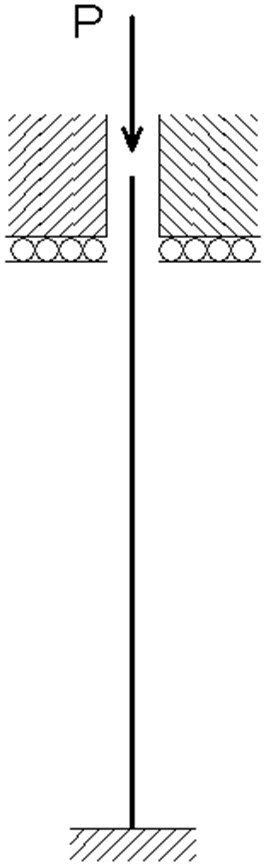
\includegraphics[width=0.1\textwidth]{UT7ej1-a}
	\label{fig:UT71.a}}
\hspace{0.1\textwidth}
\subfloat[]{
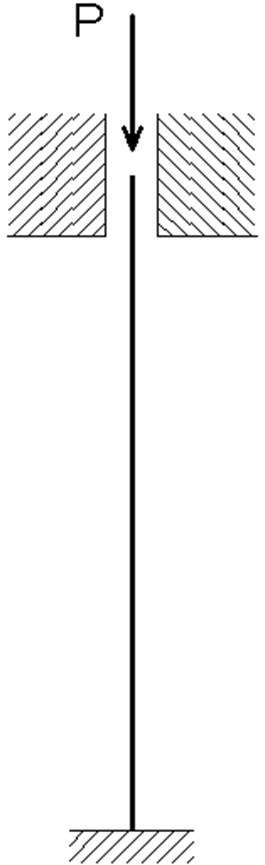
\includegraphics[width=0.1\textwidth]{UT7ej1-b}
	\label{fig:UT71.b}}
	\hspace{0.1\textwidth}
\subfloat[]{
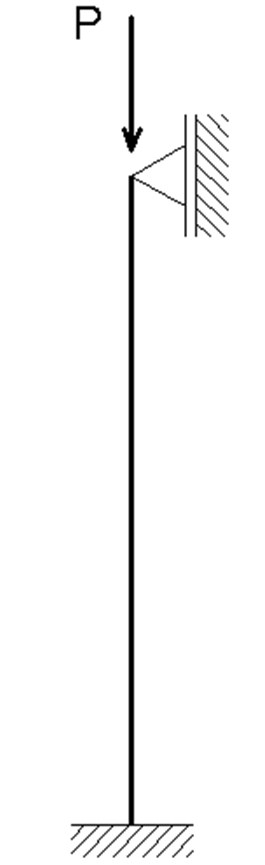
\includegraphics[width=0.1\textwidth]{UT7ej1-c}
	\label{fig:UT71.c}}
\caption{}
	\label{fig:UT71}
\end{figure}

Sugerencia: para ~\ref{fig:UT71.a} y ~\ref{fig:UT71.c}, plantear el origen de coordenadas en el extremo superior del pilar.

\ejercicio 

Dada la barra de la Figura, construida con un $PNI30$, determinar $P_{cr}$ si $\sigma_{adm}=140MPa$, $E=200GPa$ y $L=2m$.

\begin{center}
	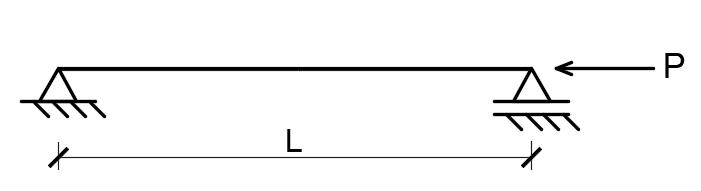
\includegraphics[width=0.5\linewidth]{UT7ej2}
\end{center}

\ejercicio 

Dimensionar la barra de la Figura en sección cuadrada de madera, sabiendo que $\sigma_{adm}=10MPa$ y $E=10GPa$. Utilizar las tablas de escuadrías de madera.

\begin{center}
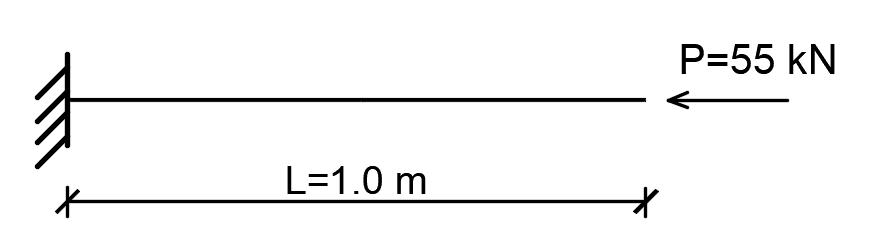
\includegraphics[width=0.5\linewidth]{UT7ej3}
\end{center}

\ejercicio 

\begin{center}
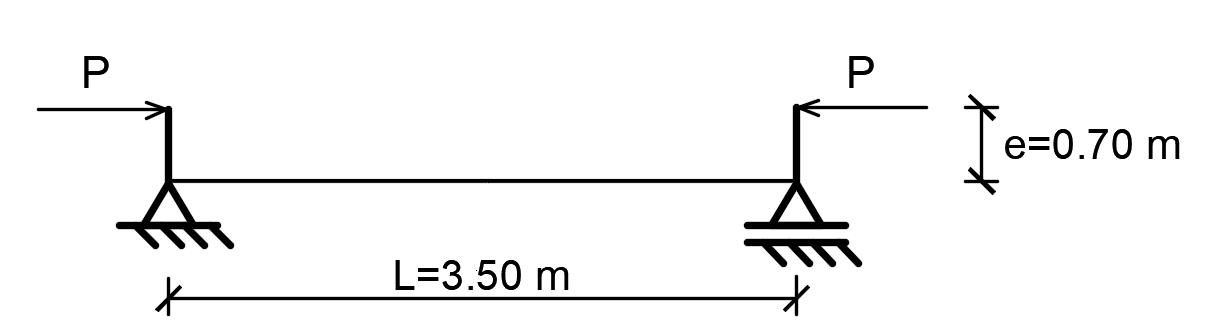
\includegraphics[width=0.6\linewidth]{UT7ej4-3}
\end{center}

Dada la barra de la estructura, construida con un $PNI14$ ($\sigma_{adm}=140MPa$ y $E=200GPa$), determinar $P_{cr}$ para los siguientes dos casos:

\begin{figure}[htb]
	\centering
\subfloat[Caso 1]{
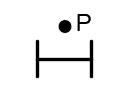
\includegraphics[width=0.2\textwidth]{UT7ej4-1}
	\label{fig:UT74.1}}
~
\subfloat[Caso 2]{
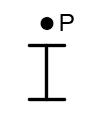
\includegraphics[width=0.15\textwidth]{UT7ej4-2}
	\label{fig:UT74.2}}
\caption{}
	\label{fig:UT74}
\end{figure}

\ejercicio

\begin{minipage}[b]{0.7\textwidth}

Una columna soldada de 8 m de luz tiene la sección de la figura conformada por acero ($\sigma_{adm}=140MPa$ y $E=200GPa$). 
\parte Hallar $x$ tal que el radio de giro de la sección según sus dos ejes sea el mismo, es decir que la sección trabaje de forma óptima.
\parte ¿Cuál es la carga de compresión crítica centrada si el esquema estructural de la columna es el de una ménsula?

\end{minipage}
~
\begin{minipage}[b]{0.3\textwidth}
\begin{center}
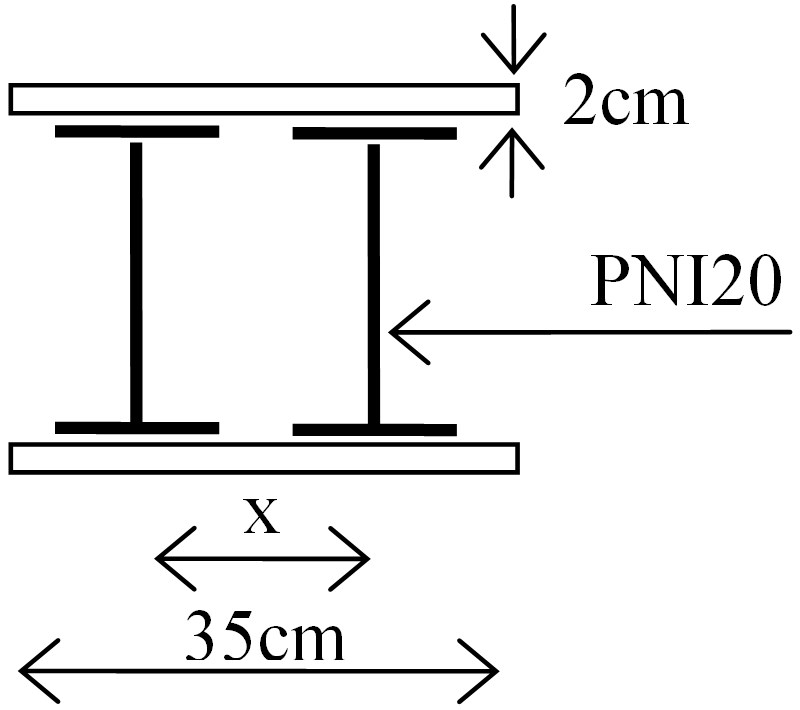
\includegraphics[width=0.85\linewidth]{UT7ej5}
\end{center}
\end{minipage}

\ejercicio

La barra horizontal de la figura está soportada por dos columnas. Cada columna está articulada en su parte superior a la barra horizontal, mientras que el apoyo inferior de la columna izquierda es un empotramiento y el de la derecha es un apoyo fijo. Ambas columnas son barras de acero $E=200GPa$ de sección transversal cuadrada con un ancho de $15 mm$.
\parte Si $a=0.4m$, ¿Cuál es el valor crítico de la carga $Q$?
\parte Si a varía entre 0 y 1 m. ¿Cuál es el valor máximo de $Q_{critico}$, y cuál es el valor correspondiente de $a$?

Nota: Estudiar la inestabilidad sólo en el plano de la figura.

\begin{center}
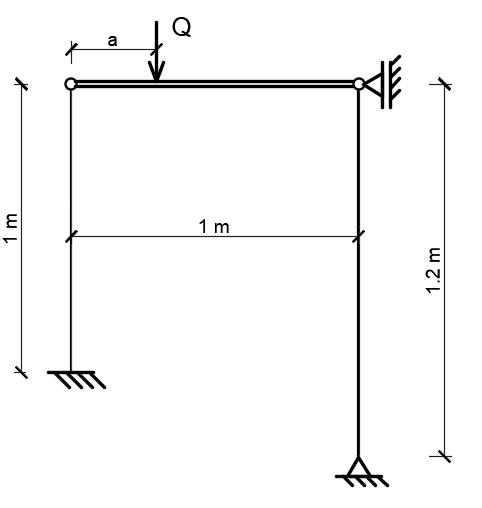
\includegraphics[width=0.4\linewidth]{UT7ej6}
\end{center}

\ejercicio

\begin{minipage}[b]{0.6\textwidth}

Una columna rectangular, con dimensiones de sección transversal $bxh$, está articulada en los extremos A y C, como se indica en la Figura.

La columna está restringida en el plano de la figura en la mitad de su altura, pero puede deformarse libremente en el plano perpendicular al de la figura.

Determinar la relación $h/b$ tal que la carga crítica sea la misma para el pandeo en los dos planos principales de la columna.

Nota: Analizar el problema a partir de los posibles modos de pandeo obtenidos en un pilar biarticulado.

\end{minipage}
~
\begin{minipage}[b]{0.4\textwidth}
\begin{center}
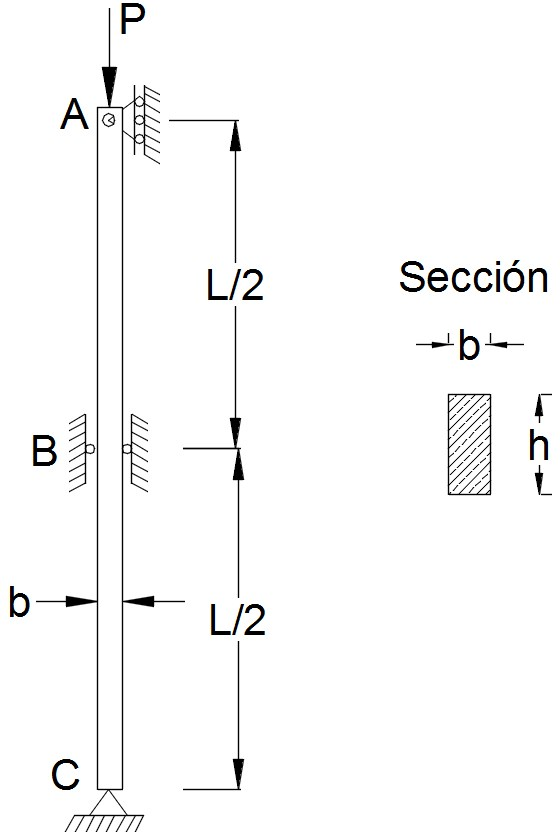
\includegraphics[width=0.65\linewidth]{UT7ej7}
\end{center}
\end{minipage}

\ejercicio

Se tiene la columna de la Figura ($EI=cte$) de largo $L$. La misma está soportada en su parte superior por un resorte elástico lineal de constante $r=2EI/L^3$ contenido en el $plano$ $xy$, mientras que en el plano perpendicular se encuentra en ménsula (libre en su extremo superior). Se pretende que la pieza sea capaz de soportar una carga $Q=200 kN$ con una altura $L=3m$.

\parte Hallar la ecuación que permite determinar la luz de pandeo en el plano del resorte y demostrar que $L_p=1,56L$. Se sugiere plantear el origen de coordenadas en el extremo superior del pilar.
\parte Dimensionar dicha pieza con un perfil laminado $PNI$ ($\sigma_{adm}=140MPa$ y $E=200GPa$).
\parte Dimensionarla utilizando perfiles laminados $PNIP$ ($\sigma_{adm}=140MPa$ y $E=200GPa$). 
\parte Dimensionarla utilizando una escuadría cuadrada de quebracho, el cual tiene una tensión admisible $\sigma_{adm,comp//}=12MPa$ (compresión paralela a las fibras) y $E=10GPa$.

En b), c) y d) indicar como orientar el perfil o escuadría.

\begin{center}
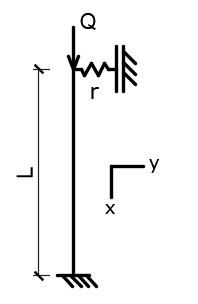
\includegraphics[width=0.2\linewidth]{UT7ej8}
\end{center}


\ejercicio (Adicional)

\begin{center}
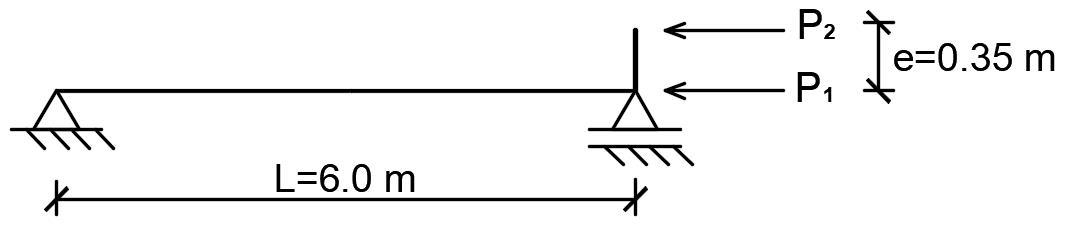
\includegraphics[width=0.6\linewidth]{UT7ej10-3}
\end{center}

Sean $P_1=500 kN$ y $P_2=120 kN$. Dimensionar en $PNIP$ (alas anchas) considerando $\sigma_{adm}=140MPa$ y $E=200GPa$. Analizar dos casos:

\begin{figure}[htb]
	\centering
\subfloat[Caso 1]{
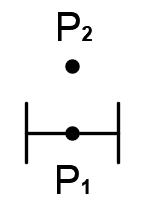
\includegraphics[width=0.15\textwidth]{UT7ej10-1}
	\label{fig:UT710.1}}
~
\subfloat[Caso 2]{
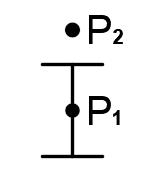
\includegraphics[width=0.15\textwidth]{UT7ej10-2}
	\label{fig:UT710.2}}
\caption{}
	\label{fig:UT710}
\end{figure}
